\documentclass[10pt]{article}
\usepackage[table]{xcolor}  % load xcolor before anything else
\usepackage[most]{tcolorbox}
\usepackage{setspace}  %line spacing
\usepackage{titling}
\usepackage{graphicx}
\usepackage{parskip}    %spaced paragraphs
\usepackage{csquotes}   %babel wanted it
% \usepackage{emptypage} % prevent page numbers and headings on empty pages
\usepackage{float} % for H specification
% \usepackage{censor}
\usepackage{amsmath}
\usepackage{fontawesome}    % fancy font special characters
% \usepackage{pdfpages} % insert pdf 
\usepackage[titletoc]{appendix}
\usepackage{pdflscape} % landscape pdf pages
\usepackage{wrapfig}
\usepackage{booktabs,nicematrix} % quality tables 

% \usepackage{tikz}
% \usepackage{circuitikz}
% \usetikzlibrary{calc}
% \usetikzlibrary{arrows,positioning}
% \usetikzlibrary{graphs, graphs.standard}

\usepackage[hang,flushmargin]{footmisc}     % footnote editing

\usepackage[font=small,labelfont=bf,justification=centering]{caption} % caption size 
\usepackage{subcaption}
\setlength{\belowcaptionskip}{-5pt}

\usepackage[hidelinks]{hyperref}  %have a review of this
\hypersetup{%
%   citecolor=black,
  colorlinks=false,
%   linkcolor=black,
%   urlcolor=black
}
\usepackage[nameinlink]{cleveref}

\usepackage{listings}% code
\definecolor{codegreen}{rgb}{0,0.6,0}
\definecolor{codegrey}{rgb}{0.5,0.5,0.5}
\definecolor{codepurple}{rgb}{0.58,0,0.82}
\definecolor{backcolour}{rgb}{0.95,0.95,0.92}
\lstdefinestyle{codestyle}{
    backgroundcolor=\color{backcolour},   
    commentstyle=\color{codegrey},
    keywordstyle=\color{blue},
    numberstyle=\tiny\color{codegrey},  % line numbers
    stringstyle=\color{codegreen},
    basicstyle=\ttfamily\lst@ifdisplaystyle\footnotesize\fi,
    breakatwhitespace=false,         % sets if automatic breaks should only happen at whitespace
    breaklines=true,                 % sets automatic line breaking
    captionpos=t,                    
    keepspaces=true,                 % keeps spaces in text, useful for keeping indentation of code (possibly needs columns=flexible)
    numbers=left,
    stepnumber=1,                    % the step between two line-numbers. If it's 1, each line will be numbered                    
    numbersep=5pt,                   % how far the line-numbers are from the code
    showspaces=false,                % show spaces everywhere adding particular underscores; it overrides 'showstringspaces'
    showstringspaces=false,          % underline spaces within strings only
    showtabs=false,                  % show tabs within strings adding particular underscores
    % tabsize=2,                       % sets default tabsize to 2 spaces
    framextopmargin=50pt,
    % title=\lstname,                  % show the filename of files included with \lstinputlisting; also try caption instead of title
    columns=fixed,                   % Using fixed column width (for e.g. nice alignment)
    frame=bottomline,
    % frame=tb,
    % belowcaptionskip=0pt,
    aboveskip=3pt,
    belowskip=3pt,
    % texcl=true,
}
\lstset{style=codestyle}

\usepackage{geometry}
\geometry{a4paper, margin=1.5cm}

\usepackage{fontspec}
\setmainfont[ 
    Mapping=tex-text,
    BoldFont={HelveticaNowText-Bold},
    ItalicFont={HelveticaNowText-RegIta},
    BoldItalicFont={HelveticaNowText-BoldItalic}
]{[HelveticaNowText-Regular]}
\usepackage{sansmath}
\sansmath

\usepackage{fancyhdr}   %footer
\fancypagestyle{myheadings}{%
    \fancyhf{}
    \renewcommand{\headrulewidth}{0.5pt}
    \renewcommand{\footrulewidth}{0pt}
    \addtolength{\headheight}{2pt}
    % \fancyhead[L]{\leftmark}
    \fancyhead[L]{ES3B2: Digital Systems Design}
    \fancyhead[R]{1922268}
    \cfoot{\thepage}
}
\pagestyle{myheadings}

\usepackage{enumitem}   %reduce list spacing
\setlist{nosep} 

\usepackage[
    backend=biber,
    style=numeric-comp,
    % style = vancouver,
    % style = science,
    % style=draft,
    % style = ieee,
    % maxnames=2, minnames=2,
    % doi=false,
    sorting=none
]{biblatex}   %bibliography
\usepackage{xurl} % break urls. load after biblatex
\addbibresource{sections/refs.bib}

\usepackage[
    separate-uncertainty=true,
    multi-part-units=single
    ]{siunitx}
\sisetup{
    detect-all,
    per-mode=symbol-or-fraction,
    tight-spacing,
    % quantity-product =,
    number-unit-product=\,,
    % space-before-unit=true
}
\DeclareSIUnit{\mAh}{mAh}

\usepackage{xltabular}
\usepackage{multirow}
\newcolumntype{Y}{>{\centering\arraybackslash}X}
\newcolumntype{Z}{>{\raggedright\arraybackslash}X}
\newcolumntype{P}[1]{>{\centering\arraybackslash}p{#1}}

\newenvironment{conditions}[1][where:]
  {#1 \begin{tabular}[t]{>{$}l<{$} @{} >{${}}c<{{}$} @{} l}}
  {\end{tabular}\\[\belowdisplayskip]}

\definecolor{titlepagecolour}{HTML}{003D99}
\definecolor{titleblue}{HTML}{1b1787} % blue
\definecolor{tableh1}{HTML}{dae3eb} %table grey
\definecolor{tableh2}{HTML}{b3ccf5} %table bluegrey
\definecolor{tableg}{HTML}{309c3d} % green
\definecolor{tablea}{HTML}{ed901f} % amber
\definecolor{tabler}{HTML}{f2422e} % red

\definecolor{hCyan}{HTML}{00FFFF}
\definecolor{hMagenta}{HTML}{FF00FF}
\definecolor{hBlue}{HTML}{0000FF}

\usepackage[british]{babel} 

% \usepackage{pgfgantt}
% \setganttlinklabel{s-s}{}
% \setganttlinklabel{f-s}{}
% \setganttlinklabel{f-f}{}

% \usepackage{titlesec} 
% \titlespacing\section{0pt}{12pt plus 4pt minus 2pt}{0pt plus 2pt minus 2pt}
% \titlespacing\subsection{0pt}{12pt plus 4pt minus 2pt}{0pt plus 2pt minus 2pt}
% \titlespacing\subsubsection{0pt}{12pt plus 4pt minus 2pt}{0pt plus 2pt minus 2pt}
% \titlespacing\paragraph{0pt}{10pt plus 4pt minus 2pt}{10pt plus 2pt minus 2pt}

\begin{document}
% \onehalfspacing
% \setstretch{1.25} % one and quarter spacing

\section{Introduction to VGA}\label{sec:intro}
VGA (Video Graphics Array) is a visual graphics standard introduced in 1987.
It was developed to work with CRT (Cathode-Ray Tube) technology, which works 
by drawing each pixel in horizontal lines vertically down the display to 
create a \emph{frame}.

In order to produce the effect of a static image 
given only a single pixel controlled per instant, the entire frame 
would be redrawn (or `refreshed') quicker than the eye can perceive.
A refresh rate of \qty{60}{\Hz} would be typical.

Due to the physical deflection of an electron beam to produce pixels, 
extra time for the beam to adjust to a new line is included in the standard, called 
the \emph{blanking interval}. 
The start of a new line is controlled by the horizontal sync (hsync) signal, with a 
new frame in turn controlled by a vertical sync (vsync) signal. The blanking intervals before 
and after these signals are respectively called the \emph{front porch} and \emph{back porch}. 
In modern standards like HDMI, this extra time has been retained and instead carries extra 
data like accompanying audio. 


\subsection{Driving the display}\label{sec:drivingdisplay}

There are four requirements for driving a VGA display:
\begin{enumerate}
    \item Clock signal driving the display signal counters.
    \item Horizontal and vertical signals, defining pixels.
    \item Drawing graphical elements to the screen.
    \item Physical video output to a display.
\end{enumerate}

\subsubsection{Clock}
The required display frequency clock can be calculated by:
\begin{align*}
    f_{\text{clock}} & = L_h \times L_v \times f_{r}
\end{align*}

\begin{conditions}
    L_h & = & horizontal lines, 1903 \\
    L_v & = & vertical lines, 931 \\
    f_{r} & = & refresh frequency, \qty{60}{\Hz} \\
\end{conditions}

% where: 
% \begin{tabular}[H]{ l c l}
%     $\lambda$ & $=$ & wavelength \\
%     $v$ & $=$ & velocity, which in this case will be $c$, the speed of light \\
%     $f$ & $=$ & frequency \\
% \end{tabular}\\

The results in a required clock frequency of \qty{106.30158}{\MHz}. 
The easiest method of producing clock signals in Verilog is to divide down the main 
processor clock to the required subdivision. In the case of the 
Nexys A7, the onboard clock is \qty{100}{\MHz} and thus cannot be divided down to 
a value that is greater. However, by using the Clocking Wizard IP provided by Xilinx, 
this can be produced. The caveat is that it will not be necessarily exact. 
In this case, the actual output clock is \qty{106.296}{\MHz}, which is within \qty{0.005}{\percent}.

\subsubsection{Signals}
In this implementation, the horizontal and vertical signals are controlled by counters 
operating at the overall display frequency, determining which pixel is being drawn. 
The counter values then determine the widths of each signal parameter.
The parameters are outlined in \cref{table:vgaparams}, which informs the display dimensions
as shown in \cref{fig:vga}.
\begin{xltabular}{\linewidth}{Y|YYYY}
    & Sync signal & Back porch & Display & Front porch \\
    \hline
    Horizontal & 151 & 384 & 1824 & 1903 \\
    \hline
    Vertical & 2 & 30 & 930 & 931 \\
    \hline
    \caption{VGA signal parameters}\label{table:vgaparams}
\end{xltabular}
The visible portion produces a display resolution of 1440x900. 

\begin{figure}[htbp]
    \centering
    \includegraphics[width=0.8\textwidth]{./figures/vga display.png}
    \caption{Display parameters}\label{fig:vga}
\end{figure}

\subsubsection{Drawing graphics}
Graphics drawing is delegated to its own module\footnote{
    \Cref{sec:drawcon}.
} separate from the VGA controller. 
To provide an overview, the graphics drawing module (draw controller) takes as input the 
current pixel by coordinates in \emph{x} and \emph{y} with reference to the top left corner
of the visible display. It outputs the colour for this pixel as a 12-bit hexadecimal number, which can then 
be passed to the VGA port.

\subsubsection{Video output}
The specifics of the output (i.e. required voltages, pin connections etc. to the D-sub connector) is
abstracted away in the constraints file for the board. In this file, the pins of the Nexys A7 
with regard to the VGA port are provided and simply need to be 
included in the compilation to be used. 

The colour channels in the port are different physical connections, taking up six pins of the 
connector - one each for red, green, and blue, in addition to each colour's ground reference. 
In the implementation for this project, the 4-bit output colour variables
(\lstinline{VGA_R}, \lstinline{VGA_G}, \lstinline{VGA_B}) 
have been merged into a single 12-bit variable (\lstinline{colour}). 

The mapping occurs as follows:

\begin{tabular}{l|lll}
    Original & \lstinline|VGA_R[3:0]| & \lstinline|VGA_G[3:0]| & \lstinline|VGA_B[3:0]| \\
    Implementation & \lstinline|colour[11:8]| & \lstinline|colour[7:4]| & \lstinline|colour[3:0]| 
\end{tabular}
% \begin{lstlisting}[numbers=none,frame=none]
%         Original        |    VGA_R[3:0]     VGA_G[3:0]      VGA_B[3:0]
%         Implementation  |    colour[11:8]   colour[7:4]     colour[3:0] 
% \end{lstlisting}

The advantage of this is that colour assignment to a pixel can now be encoded as a single hexadecimal number 
with three digits - the first encoding the red value, the second green, and the third blue. 
This is particularly useful as the encoding now follows web-safe hexadecimal colour space\footnote{
    A palette reference available at \href{https://www.rapidtables.com/web/color/Web_Safe.html}{RapidTables \faExternalLink}.
}, reducing the guesswork in developing a colour on screen.

\subsection{Limitations}
With VGA as the only display adapter available on the board, the colours available is limited 
to 4-bits for the red, green, and blue channels each. This results in 4096 total colours. 
Most modern monitor displays, on the other hand, permit over 16 million colours due to the 
use of 24-bit colour space. 

\subsection{Implementation}
The implementation of the VGA controller can be found in \cref{code:vga}.

\section{Design}
This section covers design considerations to inform subsequent development.
System specifications will be defined, and hardware purchasing will be informed.
The requirements of development will then be outlined before development commences. 

\subsection{Specification}
\label{sec:spec}
To inform design decisions, a specification of requirements will need to be 
defined, which themselves are informed by the aims in \cref{sec:aim} 
and research in \cref{sec:litrev}. This specification will cover a limited 
scope of the defined fundamentals and a selection of improvements and production,  
thereby limiting the reach of the project to ensure it remains feasible. 
This may be revisited if development is ahead of schedule. 

\subsubsection{Reporting}
The product will require a \gls{lora} radio modem and \acrshort{gps} receiver in order 
to obtain and transmit location. 

\paragraph{Timing}
\label{sec:timing}
A minimum transmission period of \qty{30}{\s} will be defined, however this 
likely can be greatly improved upon. Any gaps in live location should not be any greater 
than \qty{300}{\second}. 

\paragraph{Distance}
The tracker should be suited for, at worst case, a dense urban environment, 
and sufficiently capable to report information up to at least \qty{300}{\m},
given the roaming range of a cat\footnote{
    \Cref{sec:roam}.
} and the quoted values by competitors products\footnote{
    \Cref{sec:litsim}.
}.

\subsubsection{Portability}
With the primary target being cats, the product cannot be a significant burden to wear.
Portability in this case means four things:  
\begin{enumerate}
    \item Small form-factor.
    \item Lightweight.
    \item Battery powered.
    \item Attachable.
\end{enumerate}

\paragraph{Small form-factor}
The product needs to be small enough to fit on a cat. Given the likelihood for 
an outdoor cat to be squeezing through tight spaces, the product needs to be small 
enough to not get caught and become a restriction. 

The smallest form-factor will be aimed for, and designed in such a way 
that it can integrate in a seamless fashion with the cat's wearable 

As reasonable figure to start with would be dimensions of 
\qtyproduct{50 x 70 x 10}{\mm}.

\paragraph{Lightweight}
There is no clear answer for what an appropriate weight for the product 
would be given great range in the weight of a cat. The range easily covers
\qty{3}{\kg} to \qty{6}{\kg} for healthy pet cats \cite{kienzle:pilot}.

The answer to how much weight a cat can carry for long periods is even 
less clear. Anecdotal evidence suggests a value of around 10\%
is easily manageable. With that in mind, an aim for 
half that at, 5\% of the minimum likely weight (\qty{3}{\kg})
is a reasonable value, such that the weight is appropriate for any cat.
This puts the desired weight for the tracker at $\leq \qty{150}{\g}$, 
subject to testing to validate.

\paragraph{Battery powered}
\label{sec:specsbatt}
The key factor of portability is that the product can operate 
without a direct connection to an outlet for power. 
This means that the product requires some form of portable power.

With convenience, environmental, and energy-density (and thereby weight) considerations in mind \cite{blomgren:lithium},
the most appropriate type of battery will be rechargeable lithium-ion. This may raise some safety concerns 
due to the high likelihood of flammability of rechargeable battery cells \cite{chen:flammable}.

The most pertinent question is how long should such a battery allow the tracker to operate.
An outdoor domestic cat spends an average of \qty{8.4}{\hour} outdoors \cite{Bischof2022},
this puts a minimum value of \qty{9}{\hour} of supply necessary. 

\paragraph{Attachable}
Some method to attach the product to a cat needs to be devised. 
If it is small enough, this may be on a collar. Alternatively, 
attached to a vest may also work. This is very dependent on the 
dimensions the product takes in the end. 
Furthermore, if the product takes a prominent, protruding shape,
it needs to detach easily so as not to be a restriction for the animal.

The primary focus will be on ensuring it cannot be caught in anything to
begin with, as the tracker coming loose defeats its purpose.


\subsubsection{Suitability}
This product is designed for use by the average pet owner. Therefore, no 
specialised knowledge on how to operate any equipment can be expected. 
Furthermore, the system should be installable and maintainable using 
skills and hardware the average household can be expected to own, with some 
allowances for a small amount of DIY work. 

\paragraph{Installable}
If any hardware requires installation, it must be in as simple a manner as 
possible, with only basic (manual) tools. The expectation will be that installation
should be, at most, as difficult as a simple piece of furniture
 from a DIY store. 

\paragraph{Compliance}
Compliance for consumer products needs to be met. If certification
is not explicitly sought (for example, in the case third-party verification 
is required), the product must still meet the standards outlined such 
that it can be certified when necessary.

As a product developed in the UK, UKCA guidelines will be used. 


\subsubsection{Reliability}
The reliability of the tracker will be a matter of concern, 
as it would be especially inappropriate for it to fail in its reporting 
midway. 
\paragraph{Stable}
Part of the product relies on correct handling and processing of 
information over code. When interpreting data sets, poorly formatted 
data has the tendency to cause crashes in unsafe code. 
The code will need to be built to safely handle errors, both in the 
above-mentioned case and in any other potential points of 
software failure. 

When an error occurs, it will need to report the error and then 
continue execution with minimal downtime. Where the fault is fatal for whatever reason, 
sufficient diagnostic information is required so that fault-finding 
can be facilitated. 

\paragraph{Fault resistant}
In continuation with safely handling software errors, the 
hardware will also need to be fault-tolerant. This 
inclusively includes problems 
that may occur due to inclement weather or impacts.

\paragraph{Repairable}
Where such a hardware fault occurs that the product is no longer 
functional, repairs are to be facilitated in reasonably easy manner. 
The user should have the facilities to perform simple repairs, like 
changing an ageing battery. 
More complex repairs that require tools or specific knowledge
will be carried out by a trained individual, and therefore out of 
scope. However, a user with sufficient knowledge should not 
be hindered from performing repairs themselves if they are able. 

\paragraph{Safety}
This product introduces flammable electronics to wet environments, 
and therefore must be designed such that delicate parts are protected 
from the elements and, should such exposure occur, not be an 
inherent fire or electrocution risk.

\paragraph{Deduplication}\label{sec:dedupe}
Given that all transmissions will be operating on the same frequency, 
data from different trackers will be received by any given antenna, 
of which, the unsuitable data will need to be filtered out.  
This also brings up the question of security and `listening in' on 
another's pet. 

\subsection{System overview}
The system can be broken down into two independent parts - the `transmitter' (attached to the cat)
and `receiver' (stationary at the owner's home). Each subsystem has an independent process of operation.
The minimum requirements are subsequently outlined in \cref{fig:system overview flowchart}.

\begin{figure}[H]
    \centering
    \begin{subfigure}{.4\textwidth}
        \centering
        \begin{tikzpicture}
            \node (start) [startstop] {Start};
            \node (timer) [process, below of=start, yshift=-0.6cm] {Start timer};
            \node (loc) [process, below of=timer, yshift=-0.6cm] {Get location};
            \node (elapse) [process, below of=loc, yshift=-0.6cm] {30s elapsed};
            \node (emit) [io, below of=elapse, yshift=-0.6cm] {Emit location};

            \draw [arrow] (start) -- (timer);
            \draw [arrow] (timer) -- (loc);
            \draw [arrow] (loc) -- (elapse);
            \draw [arrow] (elapse) -- (emit);
            \draw [arrow] (emit) -- ++(2.5,0) |- (loc);
        \end{tikzpicture}
        \caption{Transmitter}
    \end{subfigure}\quad
    \begin{subfigure}{.4\textwidth}
        \centering
        \begin{tikzpicture}
            \node (start) [startstop] {Start};
            \node (inp) [io, below of=start, yshift=-0.6cm] {Await location};
            \node (store) [process, below of=inp, yshift=-0.6cm] {Store location};

            \draw [arrow] (start) -- (inp);
            \draw [arrow] (inp) -- (store);
            \draw [arrow] (store) -- ++(2.5,0) |- (inp);
        \end{tikzpicture}
        \caption{Receiver}
    \end{subfigure}    
    \caption{System overview flowchart}
    \label{fig:system overview flowchart}
\end{figure}

\subsection{Hardware}

Given the specification list, some hardware requirements can be defined to inform purchasing decisions.
The transmitter needs to be portable, therefore each component is size, weight, and power limited. The receiver,
on the other hand, is designed to be stationary and has no technical size or power limitations. However, 
it has to be sized within reason for a product designed for home use.

The following component list will help inform what specific components are required, which has been 
drawn into a hardware block diagram in \cref{fig:hardwareblockdiag} to aid visualisation. 
\begin{itemize}
    \item Transmitter
          \begin{itemize}
              \item \acrshort{gps} module for location.
              \item \gls{lora} module for transmission.
              \item Small form-factor antenna to aid transmission.
              \item Microcontroller for general computation.
              \item Battery as a remote power source.
          \end{itemize}
    \item Receiver
          \begin{itemize}
              \item \gls{lora} module for transmission.
              \item Microcontroller or \acrshort{sbc} for computation.
          \end{itemize}
\end{itemize}

% \begin{figure}[htbp]
%     \centering
%     \begin{subfigure}[b]{0.475\textwidth}
%         \centering
%         \includegraphics[height=5cm, keepaspectratio]{../figures/mcblock.png}
%         \caption{Transmitter}
%     \end{subfigure}
%     \hfill
%     \begin{subfigure}[b]{0.475\textwidth}
%         \centering
%         \includegraphics[height=5cm, keepaspectratio]{../figures/sbcblock.png}
%         % \includesvg[inkscapelatex=false,width=\textwidth]{../figures/sbcblock.svg}
%         \caption{Receiver}
%     \end{subfigure}
%     \caption{Hardware block diagram}
%     \label{fig:hardwareblockdiag}
% \end{figure}

\begin{figure}[H]
    \centering
    \begin{subfigure}[b]{0.625\textwidth}
        \centering
        
        \begin{tikzpicture}        
            \node (mc) [rec] {Microcontroller};
            \node (lora) [rec, above of=mc, yshift=0.6cm, xshift=-1.25cm] {LoRa\\module};
            \node (loraant) [rec, left of=lora, xshift=-1.5cm] {LoRa\\antenna};            
            \node (gps) [rec, above of=mc, yshift=0.6cm, xshift=1.25cm] {GPS\\module};
            \node (gpsant) [rec, right of=gps, xshift=1.5cm] {GPS\\antenna};
            \node (batt) [rec, below of=mc, yshift=-0.6cm] {Battery};

            \draw [bar] (mc) -- (lora);
            \draw [bar] (lora) -- (loraant);
            \draw [bar] (mc) -- (gps);
            \draw [bar] (gps) -- (gpsant);
            \draw [bar] (batt) -- (mc);
        \end{tikzpicture}

        \caption{Transmitter}
    \end{subfigure}
    \hfill
    \begin{subfigure}[b]{0.325\textwidth}
        \centering
        \begin{tikzpicture}        
            \node (sbc) [rec] {SBC};
            \node (lora) [rec, above of=sbc, yshift=0.6cm] {LoRa\\module};
            \node (loraant) [rec, left of=lora, xshift=-1.5cm] {LoRa\\antenna};   
            \node (pwr) [rec, below of=sbc, yshift=-0.6cm] {Mains\\power};

            \draw [bar] (sbc) -- (lora);
            \draw [bar] (lora) -- (loraant);
            \draw [bar] (pwr) -- (sbc);
        \end{tikzpicture}      

        \caption{Receiver}
    \end{subfigure}
    \caption{Hardware block diagram}
    \label{fig:hardwareblockdiag}
\end{figure}

There are many possible configurations to produce the sets of hardware required 
from parts available across different vendors. With this in mind, solutions that 
incorporate built-in features will be prioritised.

\subsubsection{SBC choices}
Some decisions were made to narrow down the diverse range of options, given hardware 
availability and technological experience. Regarding the transmitter controller;
while this may be as simple as a microcontroller, with extensibility and future-proofing 
in mind\footnote{
    For example, serving a user-interface, storing data in a database etc.
}, an \acrshort{sbc} will be the product of focus. Given hardware shortages,
should there be none available, this may be revisited. 
There are a number of \acrshort{sbc} offerings available, some of which are listed 
with a discussion in \cref{table:sbc}.

{\small
\begin{xltabular}{\linewidth}{|Z|Z|Z|Z|}
    \hline
    \rowcolor{tableh2}
    Board & Description & Benefits & Drawbacks \\
    \hline
    Raspberry Pi        & A series of general purpose \acrshortpl{sbc} using Broadcom BCM series \acrshortpl{soc}. 
        & \textbullet Inexpensive \newline \textbullet \acrshort{gpio} \newline \textbullet Pi 3 available
        & \\
    \hline
    NVIDIA Jetson Nano  & AI and neural network development focused, built around the ARM Cortex-A57 and NVIDIA Maxwell.                                       
        & \textbullet Powerful \newline \textbullet \acrshort{gpio}
        & \textbullet Expensive \newline \textbullet More powerful than necessary \newline \textbullet Availability \\ 
    \hline
    Beaglebone Black    & Pi equivalent, using an ARM Cortex-A8.                              
        & \textbullet Inexpensive \newline \textbullet \acrshort{gpio}
        & \textbullet Availability \\
    \hline
    Dell Wyse           & Thin client server/PC.
        & \textbullet Familiar interface for an end user \newline \textbullet Easier \acrshort{gui} programming  
        & \textbullet No \acrshort{gpio} \newline \textbullet Very expensive \\
    \hline
    \caption{\Acrshort{sbc} considerations}\label{table:sbc}
\end{xltabular}
}

With all things considered, the Raspberry Pi is the most obvious choice simply
from the standpoint that a Pi 3 is currently available for use. 
Given the current climate, it is virtually impossible to order computing hardware in this category. Even the Pi Compute
Modules, small form-factor Pi boards with no peripherals or breakouts, are often out of stock. This is despite the fact that 
these boards are unable to function `out of the box'. 

\subsubsection{Microcontroller choices}
The transmitter does not need to perform anything greater than obtaining \acrshort{gps} coordinates 
and transmitting them by \gls{lora} radio. For this reason, a microcontroller is well suited. 
There is an even greater selection available than with the \acrshort{sbc} choices. Therefore, 
as before, the options will be shortlisted and considered in \cref{table:mc}.
\clearpage

{\small
\begin{xltabular}{\linewidth}{|Z|Z|Z|Z|}
    \hline
    \rowcolor{tableh2}
    Board & Description & Benefits & Drawbacks \\
    \hline
    Arduino Uno & One of the most popular microcontrollers available, with an ATmega328P at its core. 
        & \textbullet Widely available \newline \textbullet Large peripheral and software support 
        & \textbullet Large \\
    \hline
    Challenger RP2040 LoRa & Embedded computer with integrated LoRa modem using the RP2040, a dual ARM Cortex-M0+ microcontroller. 
        & \textbullet Integrated \gls{lora} modem 
        & \\
    \hline
    Feather RP2040 & RP2040 board produced by Adafruit in the feather form-factor.
        & \textbullet Feather form-factor \newline \textbullet USB-C
        & \\
    \hline
    Wio-E5 mini & Compact LoRa dev board produced by Seeed Studio using an STM32WLE5JC, a bundled ARM Cortex-M4 microcontroller and SX126X \gls{lora} radio modem.
        & \textbullet Integrated microcontroller and \gls{lora} modem \newline \textbullet USB-C
        & \textbullet Availability \newline \textbullet Involved programming requirements\\
    \hline
    Feather 32u4 with LoRa & Feather form-factor board with LoRa produced by Adafruit, sporting an ATmega32u4.
        & \textbullet Integrated \gls{lora} modem \newline \textbullet Prior experience \newline \textbullet Feather form-factor
        & \textbullet Availability \\
    \hline
    \caption{Microcontroller considerations}\label{table:mc}
\end{xltabular}
}

The board of choice here would be the Feather RP2040. While integrated \gls{lora} 
is certainly beneficial, having the flexibility to customise it during development 
may prove more helpful\footnote{
    The RFM95W \gls{lora} chipset uses \acrshort{spi} and has, in previous experience,
caused difficulties with hardware on the same bus. In case it is necessary, an alternative set
of hardware using the \acrshort{i2c} bus will be produced.
}. Furthermore, this board shares the advantage of other Feather 
boards in that they are stackable, meaning Adafruit's large range of peripherals 
(including \gls{lora} Featherwings and \acrshort{gps} Featherwings) are available to use. 

Purchasing two such \gls{lora} Featherwings for use in the transmitter and receiver 
ensures they are able to communicate with each other without issue. Given the selected 
form-factor and subsequent ease of use, it follows that the \acrshort{gps} module will be 
from Adafruit's Featherwing line. 

\subsection{Purchasing}

Some antenna options will be included as the best approach 
for this has not yet been determined. Ceramic antennae have the smallest form-factor,
however they may prove difficult to mount due to small contact points compared to more traditional 
wire antennae. The receiver will also require a large gain antenna to pick up weak transmissions.

A preliminary hardware set was produced\footnote{
    \Cref{table:prelimhardwarelist}.
}. This list consists 
of two sets of hardware for the transmitter, hardware required regardless of set, and some antenna 
options. 

The radios selected use the same model modem, the RFM95W \cite{hoperf:rfm95w}, 
ensuring the modules are capable of communicating (i.e. are operating within the 
same wavelength range).

\paragraph{Order review}
The list had to be adjusted to primarily target hardware from approved vendors\footnote{
    \Cref{table:updatedhardwarelist}.
}. 
With the vendor adjustment made, some of the initial hardware had to be substituted for 
more expensive alternatives. This made board options simpler by limited the feasible solution
to a Feather M0 with bundled \gls{lora} modem. Additional accessories were included, along with 
an extensive set of antenna and battery options to choose from. 

This list was further adjusted to omit spare hardware that is available to use (for example, 
headers, connectors, etc.). Furthermore, battery purchasing will be put on hold until 
the required capacity can be determined. Finally, the \gls{lora} module for the Pi was 
changed to a \acrshort{hat}. This uses the same radio hardware, but has the additional benefit 
of being able to directly interface with the Pi pins. 
The list was then requested for purchasing. 




\section{Testing and verification process}\label{sec:test}
Testing designs before compiling them becomes ever more important as complexity scales. 
In the later stages of the project, a single compilation could take as much as ten minutes, 
highly restricting iterative testing methodologies like divide and conquer\footnote{
    A methodology where debugging statements are printed to console to narrow down the source of a problem.
    Highly reliant on running many test suites in quick succession. 
}. Therefore, the importance of testing via simulations is emphasised. 

To illustrate this process, an example will be outlined. Following an agile-like development methodology 
for this project prioritised producing functional code as quickly as possible. 
For static but repeatable elements, this means a large amount of hardcoded software, 
making the code unwieldy and increasing the difficulty maintaining the codebase.
To improve this, the logic can be synthesised from a FOR loop instead. 

\subsection{The hardcode}
\begin{lstlisting}
initial begin
    colourspace[0] <= 12'hfff;
    colourspace[1] <= 12'hfdf;
    colourspace[2] <= 12'hfbf;
    ... 
    colourspace[7] <= 12'f1f;
    colourspace[8] <= 12'dff;
    ... 
    colourspace[63] <= 12'h11f;
end
\end{lstlisting}
This was generated from the following Python script (modified slightly for clarity):
\begin{lstlisting}[language=Python]
    r = 15
    g = 15
    b = 15
    for count in range(0,64):
        print(f"colorspace[{count}] <= 12'h{r:x}{g:x}{b:x};")
        g = g - 2
        if(g < 0):
            r = r - 2
            g = 15
\end{lstlisting}

\subsection{Rewrite in Verilog}
The hardcoded logic can be synthesised from a FOR loop, written in Verilog directly in this case.
This is almost a direct translation from the Python script to Verilog, however there are a number of differences. 
Since the code does not need to be printed to be copied, that stage is omitted entirely. Instead, the assignment of the 
colour to \lstinline|colourspace| is made directly through an intermediary variable \lstinline|tcol|, 
which is made of the \lstinline|r|, \lstinline|g|, and \lstinline|b| bitshifted to their respective places.
\begin{lstlisting}[language=Verilog]
for(i=0;i<64;i=i+1)begin
    tcol = r<<8;
    tcol = tcol + g<<4;
    tcol = tcol + b;
    colourspace[i] = tcol;
    g = g - 2;
    if(g < 1) begin
        r = r - 2;
        g = 4'hf;
    end
end
\end{lstlisting}
This can then be run in a test bench to see the resultant values of
\lstinline|tcol|, \lstinline|r|, \lstinline|g|, \lstinline|b|, and \lstinline|colourspace|.
\begin{figure}[H]
    \centering
    \includegraphics[width=\textwidth]{figures/tb/1.png}
\end{figure}
The resulting colour values are not quite correct, with the red value stuck at 0.

\begin{minipage}{0.475\linewidth}
\begin{lstlisting}[language=Verilog]
for(i=0;i<64;i=i+1)begin
    colourspace[i] = r<<8 + g<<4 + b;
    g = g - 4'h2;
    if(g < 4'h1) begin
        r = r - 4'h2;
        g = 4'hf;
    end
end    
\end{lstlisting}
\end{minipage}\hfill
\begin{minipage}{0.5\linewidth}
    \centering
    \includegraphics[width=\linewidth]{figures/tb/2.png}
\end{minipage}
This attempts to perform the bit-shift in a single line, however the end result is all 0.
The intermediary variable is necessary. 

\begin{minipage}{0.475\linewidth}
\begin{lstlisting}[language=Verilog]
for(i=0;i<64;i=i+1)begin
    tcol = tcol + g<<4;
    tcol = tcol + b;
    colourspace[i] = tcol;
    g = g - 4'h2;
    if(g < 4'h1) begin
        r = r - 4'h2;
        g = 4'hf;
    end
end
\end{lstlisting}
\end{minipage}\hfill
\begin{minipage}{0.5\linewidth}
    \centering
    \includegraphics[width=\linewidth]{figures/tb/3.png}
\end{minipage}
This indicates the red bit-shift is always returning 0 and non-functional. 
The gradient produced is also not what is intended. It may be better to move 
to subtracting a constant value. 

\begin{minipage}{0.475\linewidth}
\begin{lstlisting}[language=Verilog]
for(i=0;i<64;i=i+1)begin
    colourspace[i] = tcol;
    tcol = tcol - 12'h020;
    if(tcol[7:4] < 4'h1) begin
        tcol = tcol - 12'h200;
    end
end
\end{lstlisting}
\end{minipage}\hfill
\begin{minipage}{0.5\linewidth}
    \centering
    \includegraphics[width=\linewidth]{figures/tb/4.png}
\end{minipage}
This subtractive method appears better, however the aim is to drop the red value by two, whereas here it only drops by one.
The loop in an \lstinline|initial| block does not appear to be synthesised correctly for actual implementation, resulting
in a black screen.

\begin{minipage}{0.475\linewidth}
\begin{lstlisting}[language=Verilog]
for(i=0;i<64;i=i+1)begin
    colourspace[i] = tcol;
    tcol = tcol - 12'h020;
    if(tcol[7:4] < 4'h1) begin
        tcol = tcol - 12'h500;
    end
end 
\end{lstlisting}
\end{minipage}\hfill
\begin{minipage}{0.5\linewidth}
    \centering
    \includegraphics[width=0.9\linewidth]{figures/tb/5.png}
\end{minipage}
The code was moved to an \lstinline|always| block to allow it to be synthesised to the display correctly. 
Furthermore, the reduction was increased. The test bench shows the value stay the same - the 
IF statement is not evaluating true since \lstinline|tcol[7:4]| will move from 1 to F. 

\begin{minipage}{0.475\linewidth}
\begin{lstlisting}[language=Verilog]
for(i=0;i<64;i=i+1)begin
    colourspace[i] = tcol;
    tcol = tcol - 12'h020;
    if(tcol[7:4] == 4'hf) begin
        tcol = tcol - 12'h100;
    end
end 
\end{lstlisting}
\end{minipage}\hfill
\begin{minipage}{0.5\linewidth}
    \centering
    \includegraphics[width=0.9\linewidth]{figures/tb/6.png}
\end{minipage}
The values are now reducing in the correct progression. 

\section{Conclusion}

\subsection{Evaluation}
The designed game will be evaluated against the criteria. 
\paragraph{User control}
The user takes control of a reticle to select a colour, which is controllable
by tilting the board in the desired movement direction. The sprite is 
bounded within the selection area. 
\paragraph{Object interactions} 
The game progresses by clearing the screen by progressively selecting colours. 
The grid items need to effectively interact with each other in order to determine 
adjacency and when a grid has been matched to the selected colour. However, 
some visual artefacts may occur. 
The player sprite also interacts with the selection grid underneath to select a 
colour and assumes the characteristics of transparency. 
\paragraph{Info bar}
An info bar is drawn from the graphics controller as a banner at the topmost
hierarchical layer, and includes sprites for the game title and IDs. 
\paragraph{Extra hardware}
The game makes use of the in-built accelerometer, available on the SPI interface,
in order to control player movement. It also displays the game title on the 7-segment display. 
\paragraph{Sprites}
The game makes use of 3 sprites, one for the player, title, and IDs. 
There are some issues with the player sprite appearance, where the sprite is shifted somewhat. 
However, these have been mitigated by adjusting the sprite ROM to negate this effect.

\subsection{Reflection} 

\paragraph{Colour blindness support}
The game in its current form is not supportive of most forms of colour vision deficiency, with the likely exception of 
tritanopia and tritanomoly. Support can be increased by adjusting the colour space used, i.e. using a 
Cividis or Viridis colour space \cite{Nunez2018}, or allowing different colour selections by the player.

Support for achromatopsia may prove difficult while retaining game flow and simplicity. One possible solution is 
to use symbolic elements on cells, and improve the animation between cells to indicate matching. This would, however, 
require a significant redesign of the game logic. 

\subsubsection{Player comments}
During player testing, a notable complaint that cropped up was the difficulty of matching a colour,
with the controls feeling `slippery' and `imprecise'. 
This issue can be broken down into two parts - difficulty in identifying the colour to match, and moving to that colour. 
\paragraph{Identification} With the 64 colour selection, differentiating tones in the same quadrant 
can prove difficult. Colour definition can be improved with a greater display resolution, perhaps by moving 
to a more up-to-date display standard, although this would require the requisite adapter to be available on the board. 
\paragraph{Movement} Movement is altogether both too responsive and not responsive enough. This makes fine adjustments
difficult and overshoots frequent. Overshoots can be improved with the current accelerometer implementation 
by compressing the responsive range to cover half the rotation it does currently. In other words, rather than a complete 
half turn returning 16 (the greatest value), only a quarter turn is needed, with every second value skipped. The 
downside is that fine adjustments will be made more difficult. A complete reimplementation of the accelerometer 
will be needed to return data in finer intervals to combat this. 

\subsubsection{General comments}
The development process for the game was not smooth. Debugging, especially for graphical glitches or 
player interactions, proved particularly difficult to manage. 
This is due to how they cannot be observed easily within test benches. Some issues also 
do not appear to be problematic in test benches, whereas fail to render in actual implementation. 
The final implementation also suffers some logical glitches, where a cell remains unmatched. Overall,
the game functions fairly well otherwise. 

\nocite{digilentmanual}

\printbibliography

\clearpage
\begin{appendices}
\pagenumbering{Roman}

\chapter{Further Reading}
\printbibliography[heading=none,notcategory=cited]

\chapter{Pinout Diagrams}

\vfill

\begin{figure}[H]
    \centering
    \includegraphics[width=0.5\textwidth]{../figures/raspberry-pi-pinout.png}
    \caption[Raspberry Pi pinout]{Raspberry Pi pinout, available at \href{https://pinout.xyz}{pinout.xyz \faExternalLink}}
    \label{fig:raspipinout}
\end{figure}

\vfill

\begin{figure}[H]
    \centering
    \includegraphics[width=\textwidth]{../figures/featherm0pinout.png}
    \caption[LoRa Feather M0 pinout]{\gls{lora} Feather M0 pinout \cite{img:m0}}
    \label{fig:m0pinout}
\end{figure}

\vfill

\begin{figure}[H]        
    \centering
    \begin{subfigure}[b]{0.35\textwidth}
        \centering
        \includegraphics[angle=90,width=\textwidth,height=6cm, keepaspectratio]{../figures/gpspins.jpg}
        \caption{GPS Featherwing pins}
        \label{fig:gpspin}
    \end{subfigure}
    \hfill
    \begin{subfigure}[b]{0.6\textwidth}  
        \centering 
        \includegraphics[height=6cm,width=\textwidth, keepaspectratio]{../figures/gpsstack.jpg}
        \caption{GPS Featherwing stacked}
        \label{fig:gpstack}
    \end{subfigure}  
    \caption[GPS Featherwing pin images]{GPS Featherwing pin images, available at \href{https://www.adafruit.com/product/3133}{Adafruit \faExternalLink}}    
    \label{fig:gpspins}     
\end{figure}

\href{https://learn.adafruit.com/adafruit-ultimate-gps-featherwing/pinouts}{GPS Featherwing pinouts reference link \faExternalLink}

\vfill

\chapter{Case design}
    
\vfill
    \begin{figure}[H]
        \caption[First case print]{First case print, showing various angles}         
        \label{fig:case1img}
        \centering
        \begin{subfigure}[b]{0.4\textwidth}
            \centering
            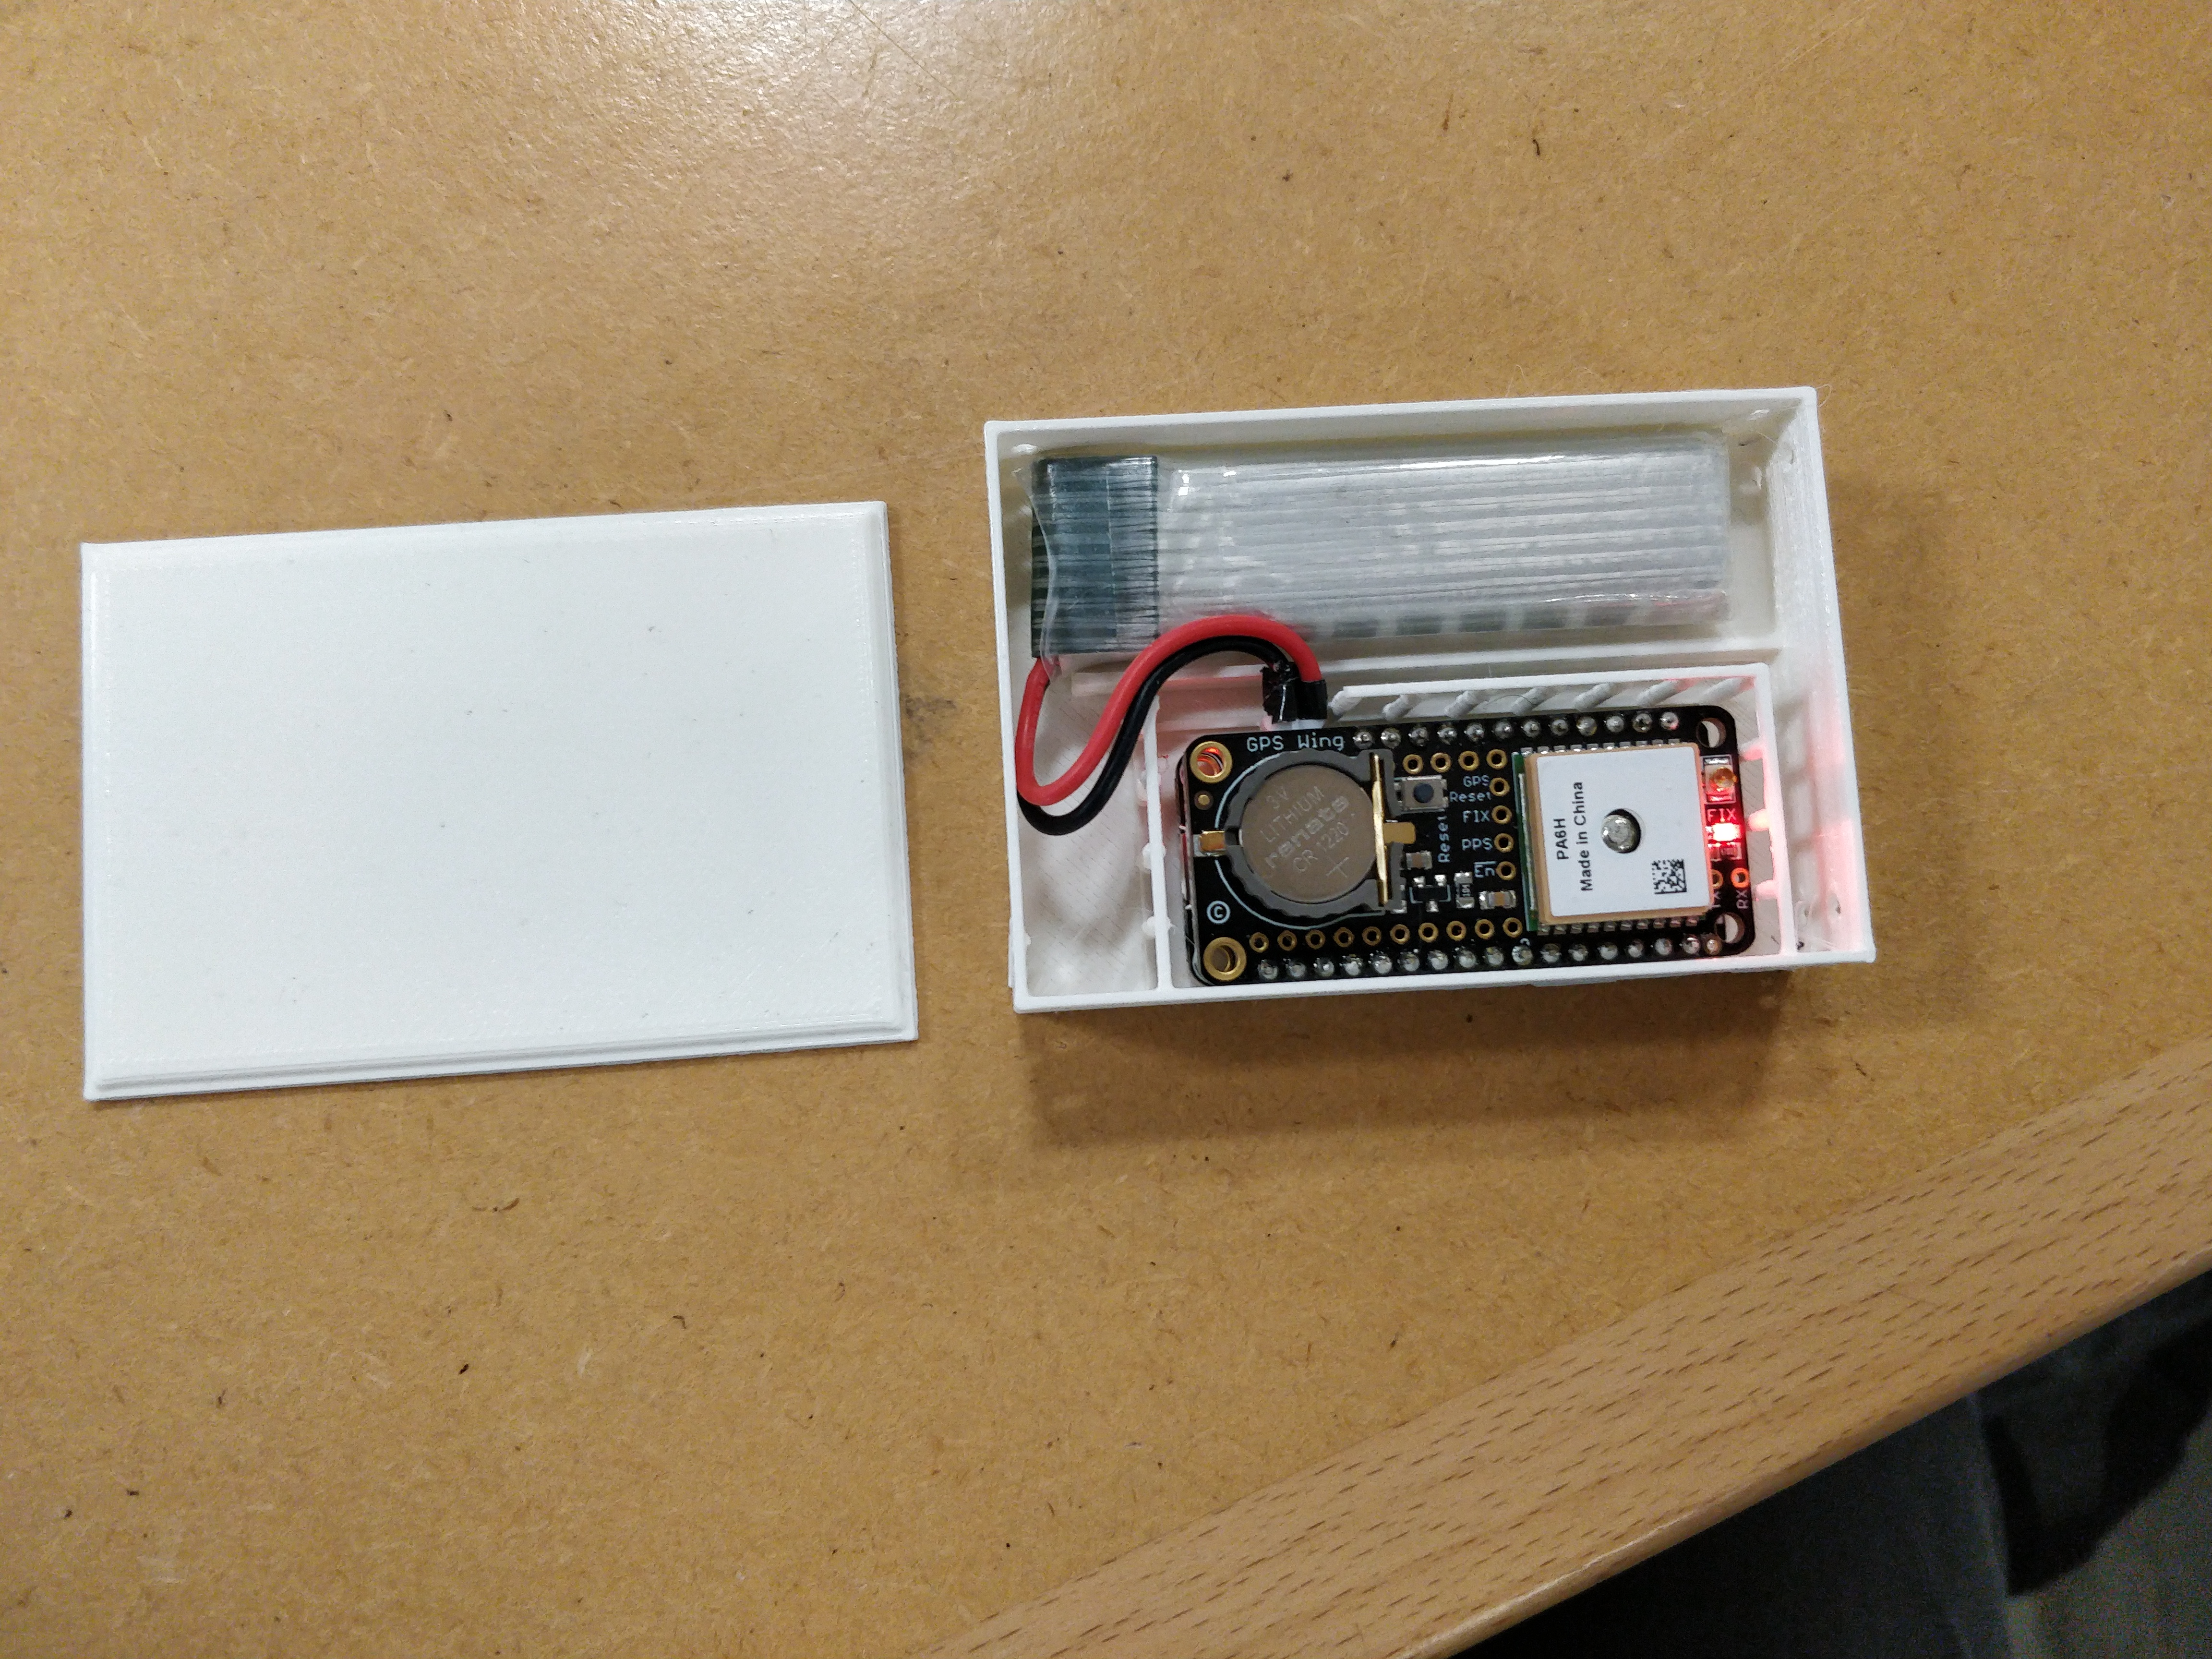
\includegraphics[angle=90,width=\textwidth]{../figures/Pics/firstcase1.jpg}
            \caption{Case overview with lid}
        \end{subfigure}
        \hfill
        \begin{subfigure}[b]{0.4\textwidth}  
            \centering 
            \includegraphics[width=\textwidth]{../figures/Pics/firstcase2.jpg}
            \caption{Battery port view}
        \end{subfigure}
        \vskip\baselineskip
        \begin{subfigure}[b]{0.4\textwidth}   
            \centering 
            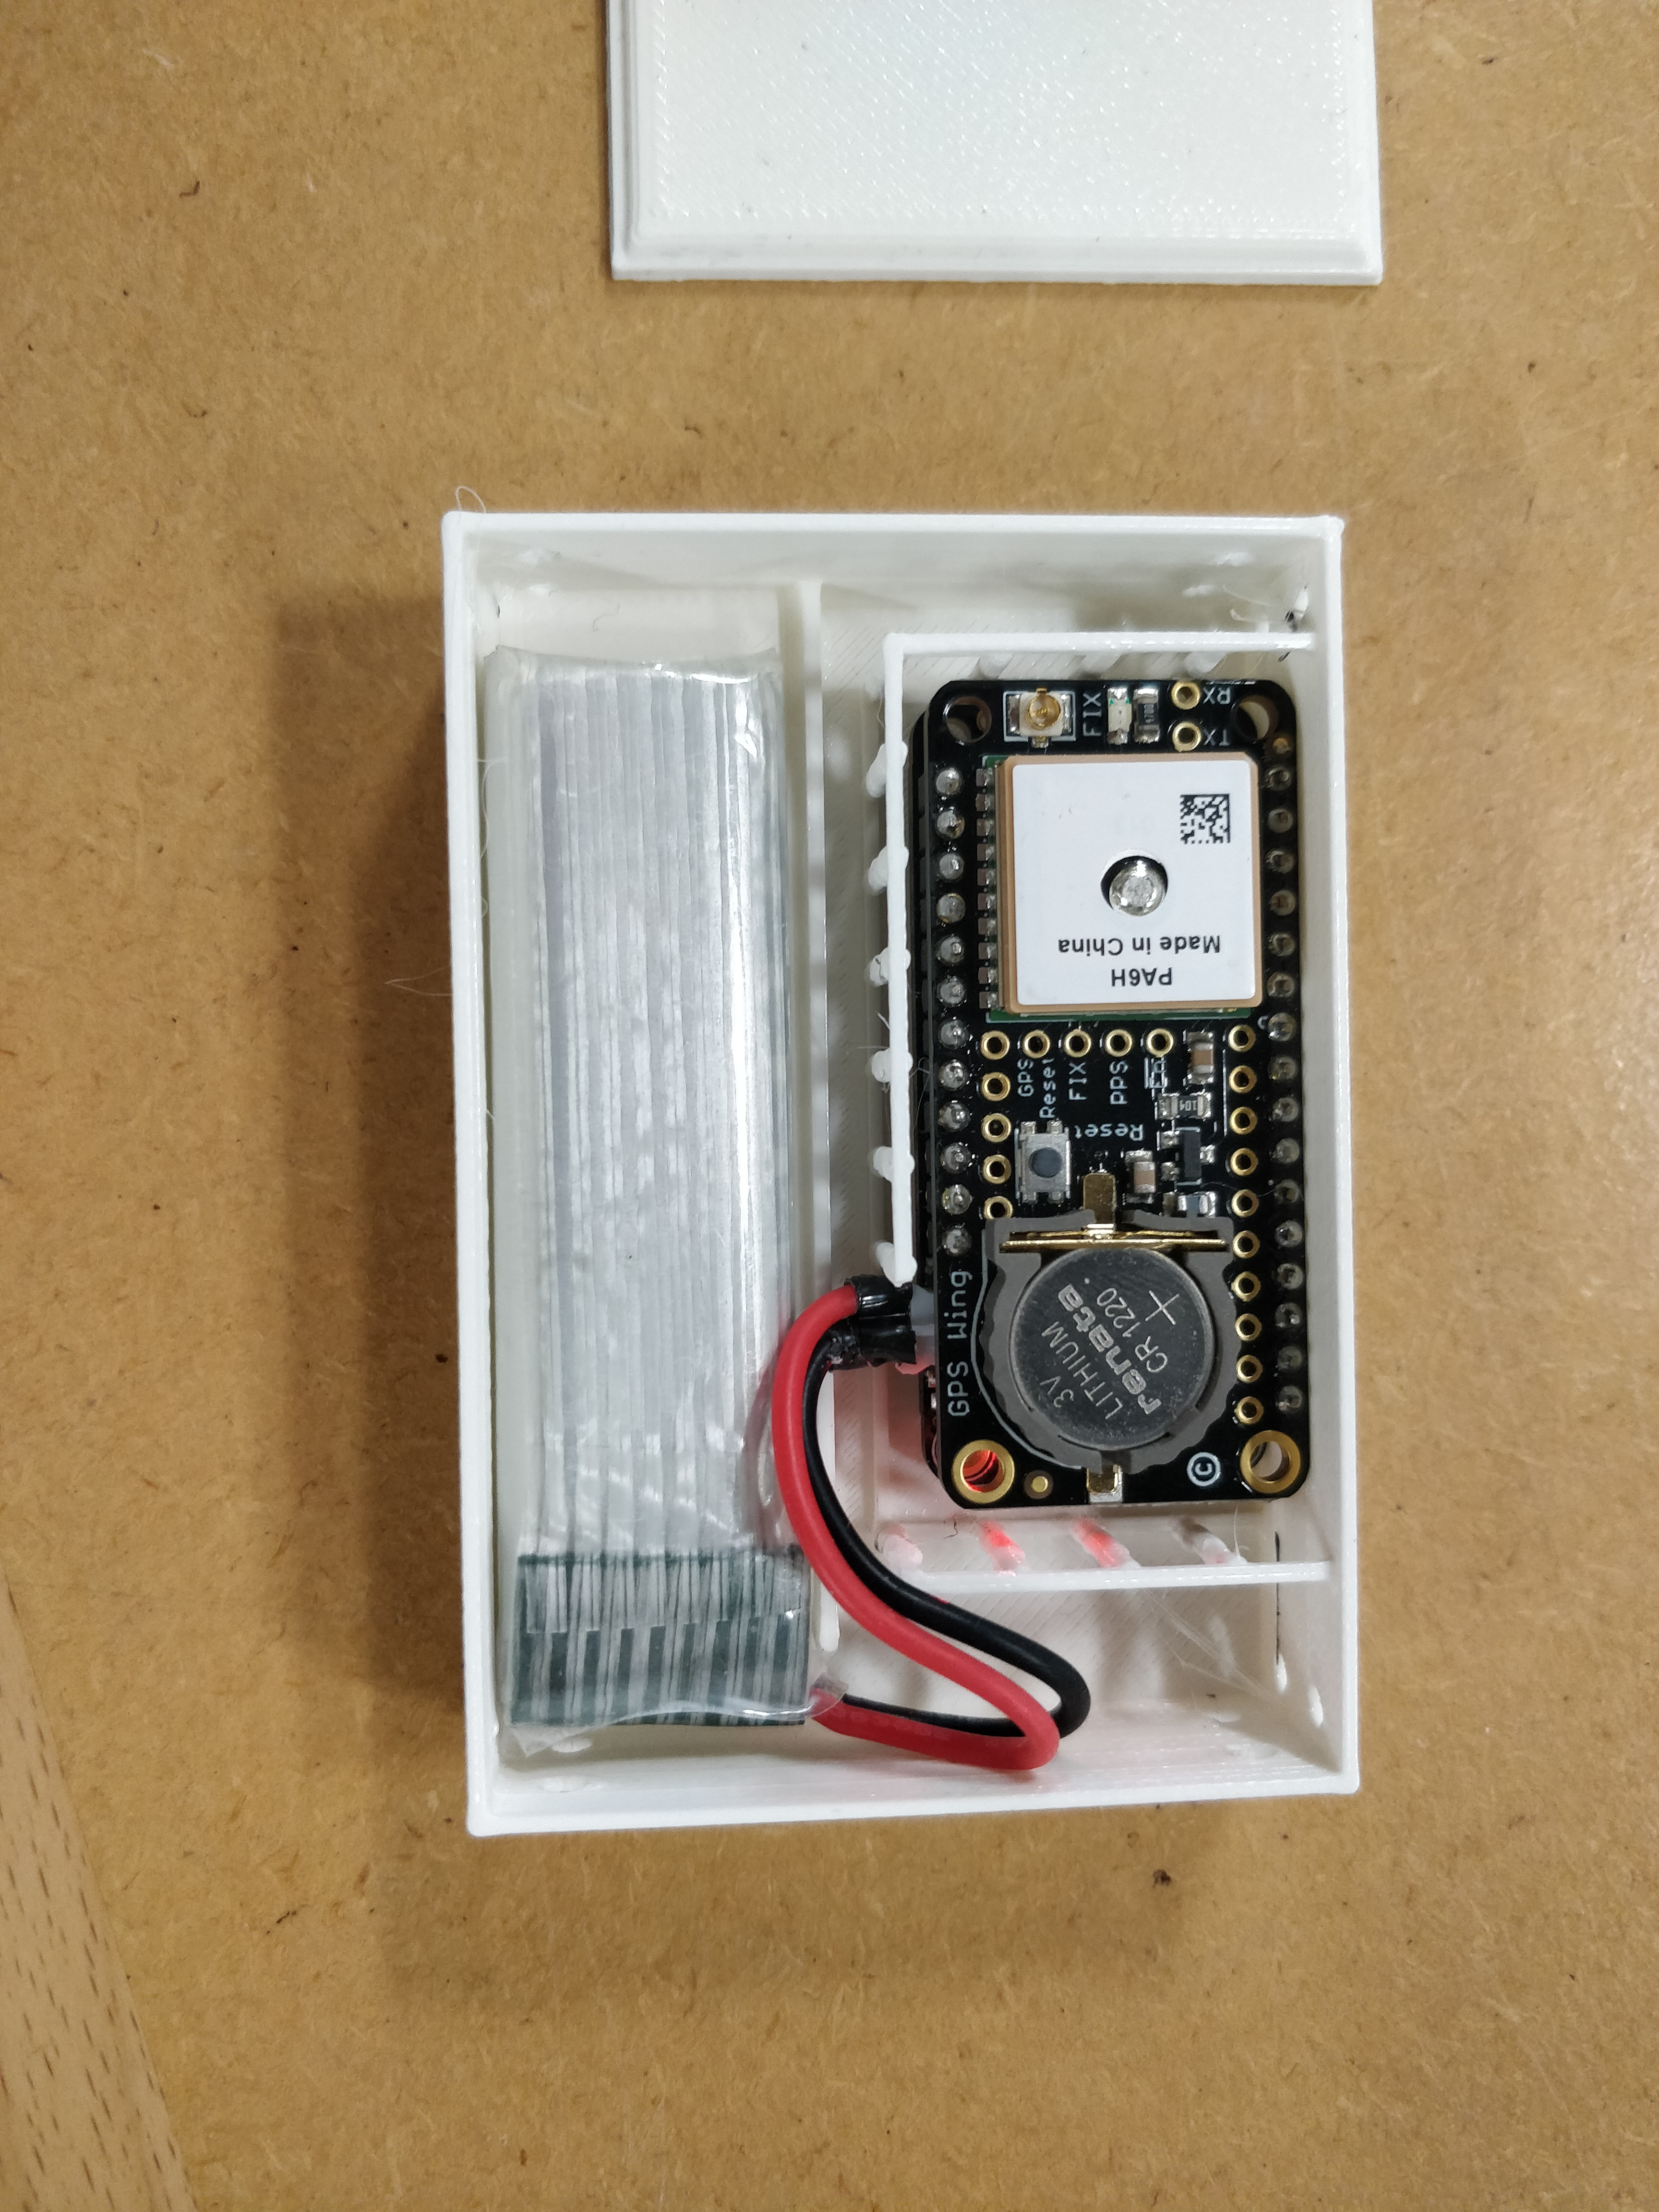
\includegraphics[width=\textwidth]{../figures/Pics/firstcase3.jpg}
            \caption{Top view}            
            \label{fig:case1top}
        \end{subfigure}
        \hfill
        \begin{subfigure}[b]{0.4\textwidth}   
            \centering 
            \includegraphics[width=\textwidth]{../figures/Pics/firstcase4.jpg}
            \caption{Angled front view}
        \end{subfigure}        
    \end{figure}
    \vfill
    \clearpage

    % \begin{figure}[H]        
    %     \label{case1dwg}
    %     \caption{Case 1 dimensional drawing}
    %     \includegraphics[angle=-90,width=\textwidth]{../../Design/case1.pdf}
    % \end{figure}  

    % \includepdf[pagecommand={},angle=-90,scale=0.9,pagecommand=\section{Case 1 dimensional drawing \label{fig:case1dwg}}]{../../Design/case1.pdf}  
    
    \begin{figure}[H]      
        \caption{Case 1 dimensional drawings}
        \includepdf[pagecommand={},angle=-90,scale=0.9]{../../Design/case1.pdf}  
        \label{fig:case1dwg}
    \end{figure}
    % \clearpage
       
    % \section{Case 2 images}
    \vfill
    \begin{figure}[H]          
        \caption[Second case print]{Second case print, showing various angles} 
        \label{fig:case2img}  
        \centering
        \begin{subfigure}[b]{0.6\textwidth}  
            \centering 
            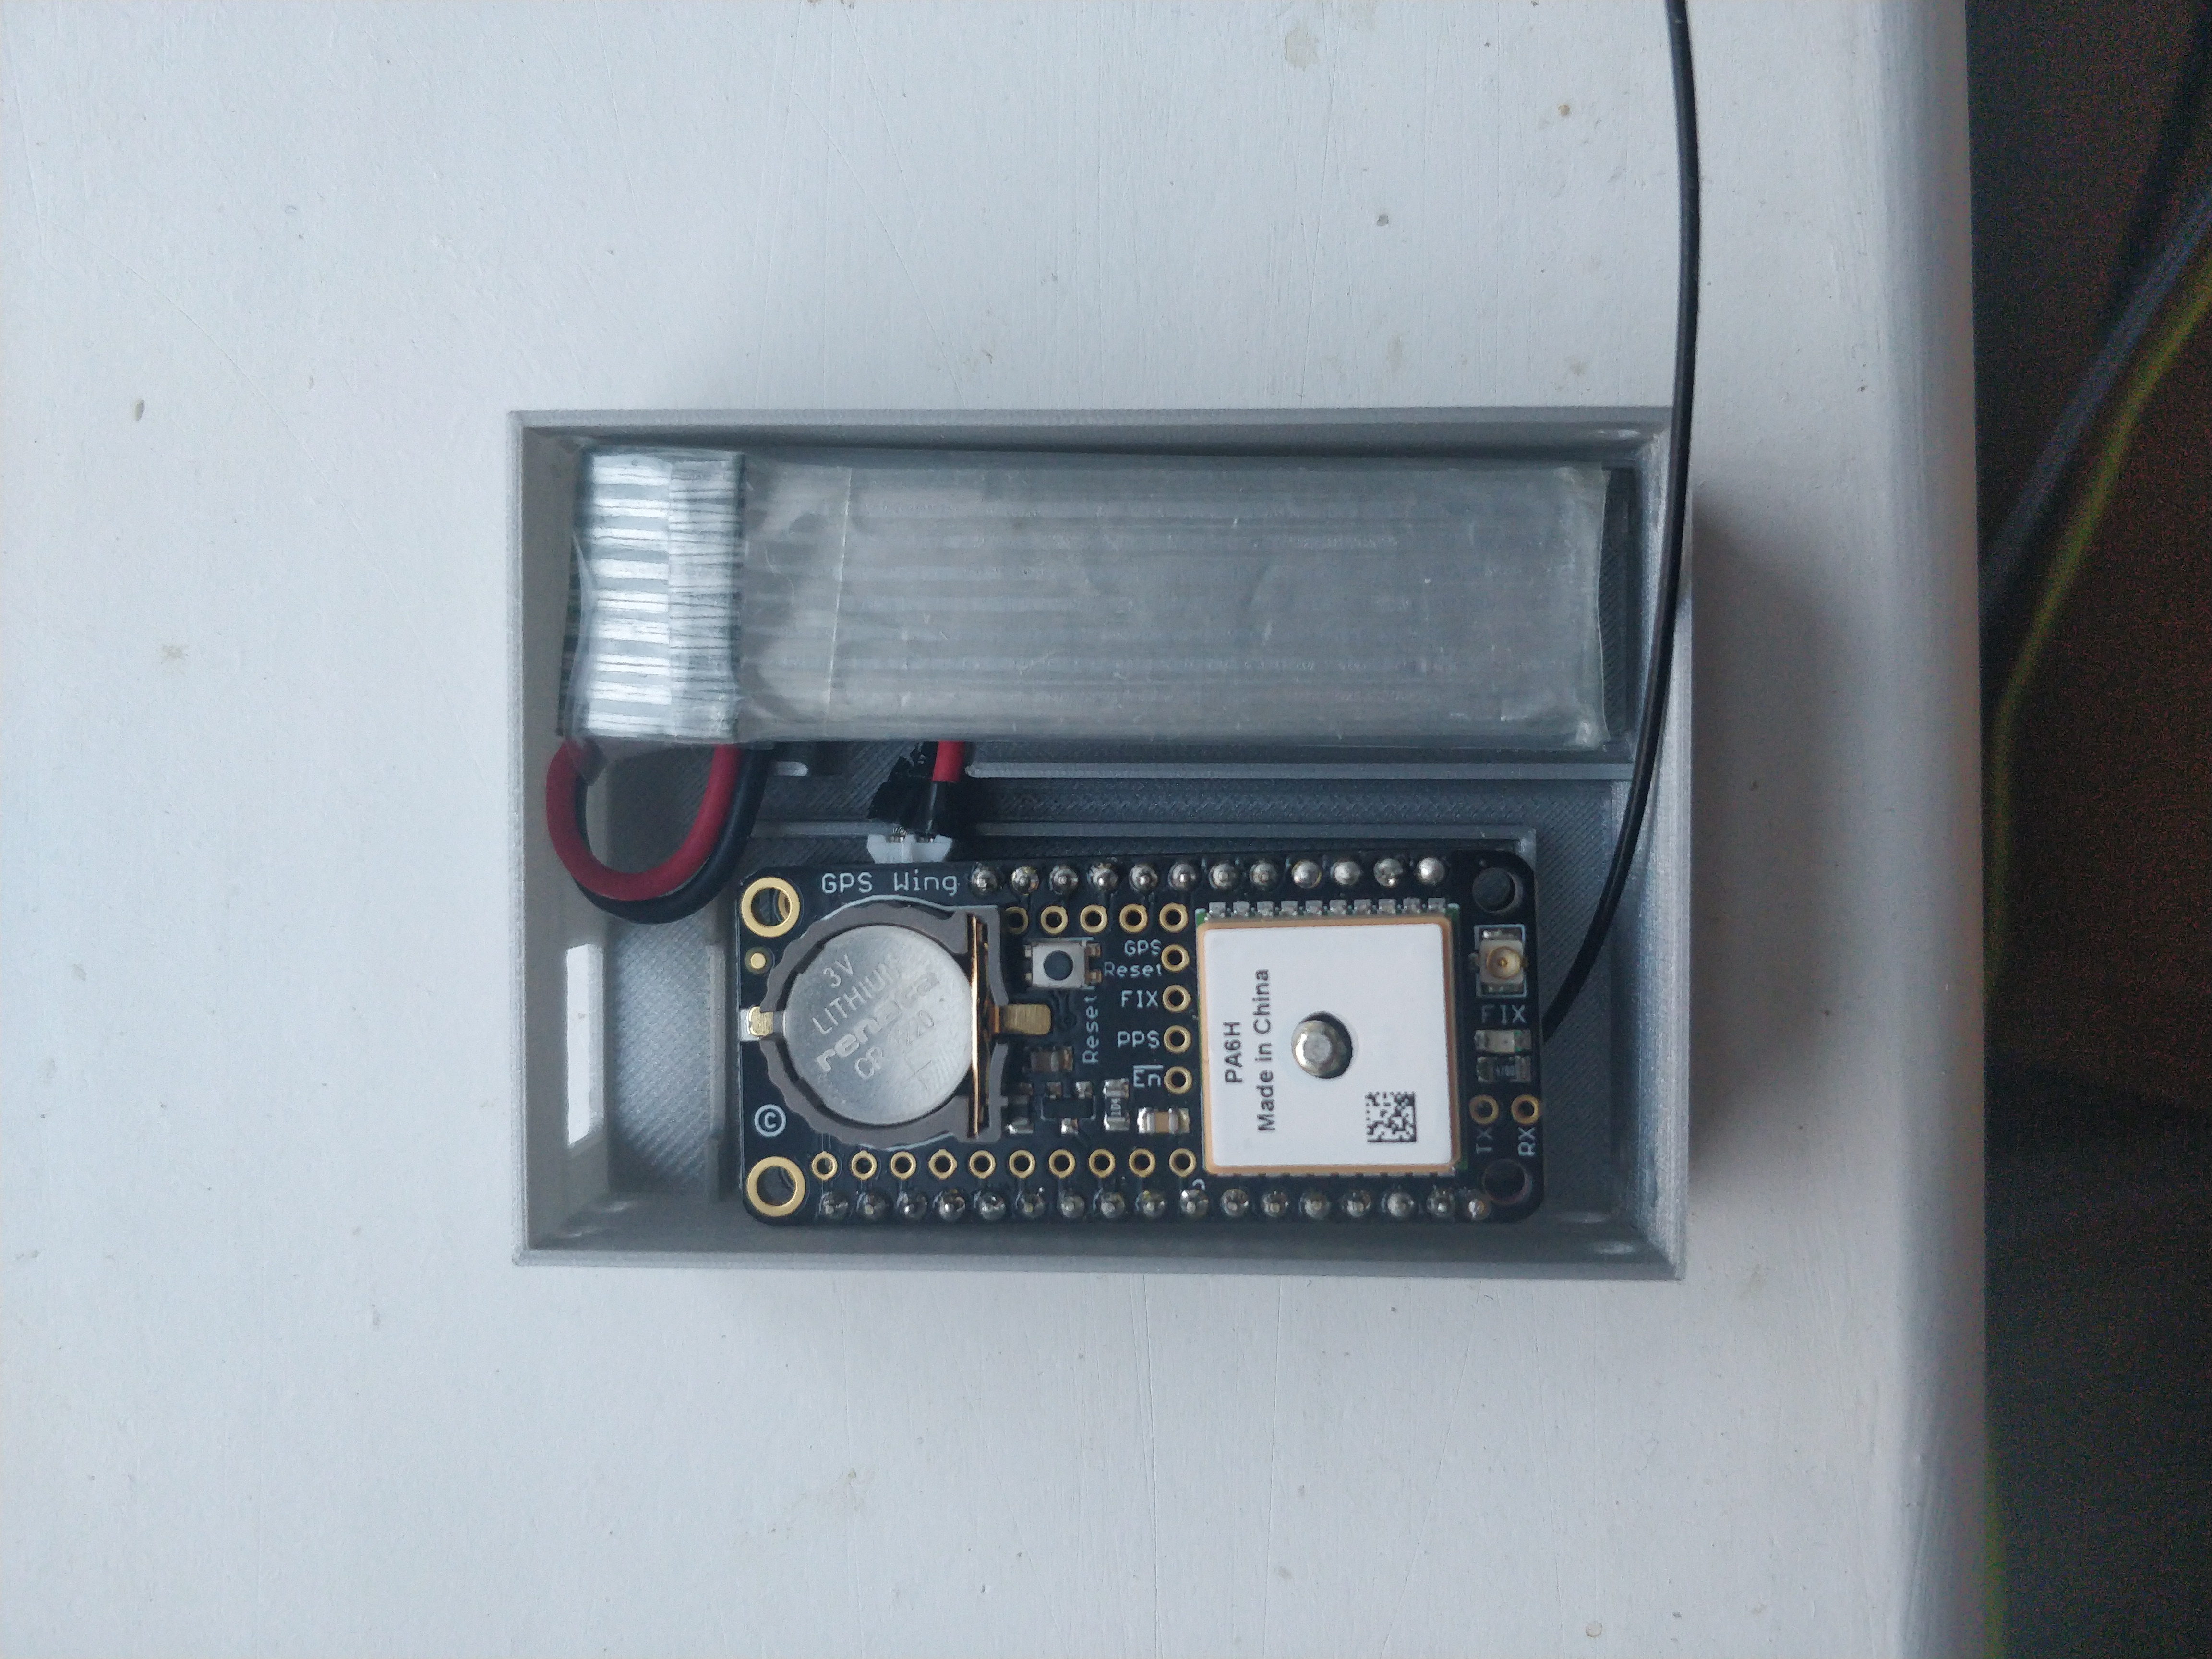
\includegraphics[width=\textwidth]{../figures/Pics/secondcase0.jpg}
            \caption{Case overview}
        \end{subfigure}
        \vskip\baselineskip
        \hspace*{\fill}
        \begin{subfigure}[b]{0.3\textwidth}
            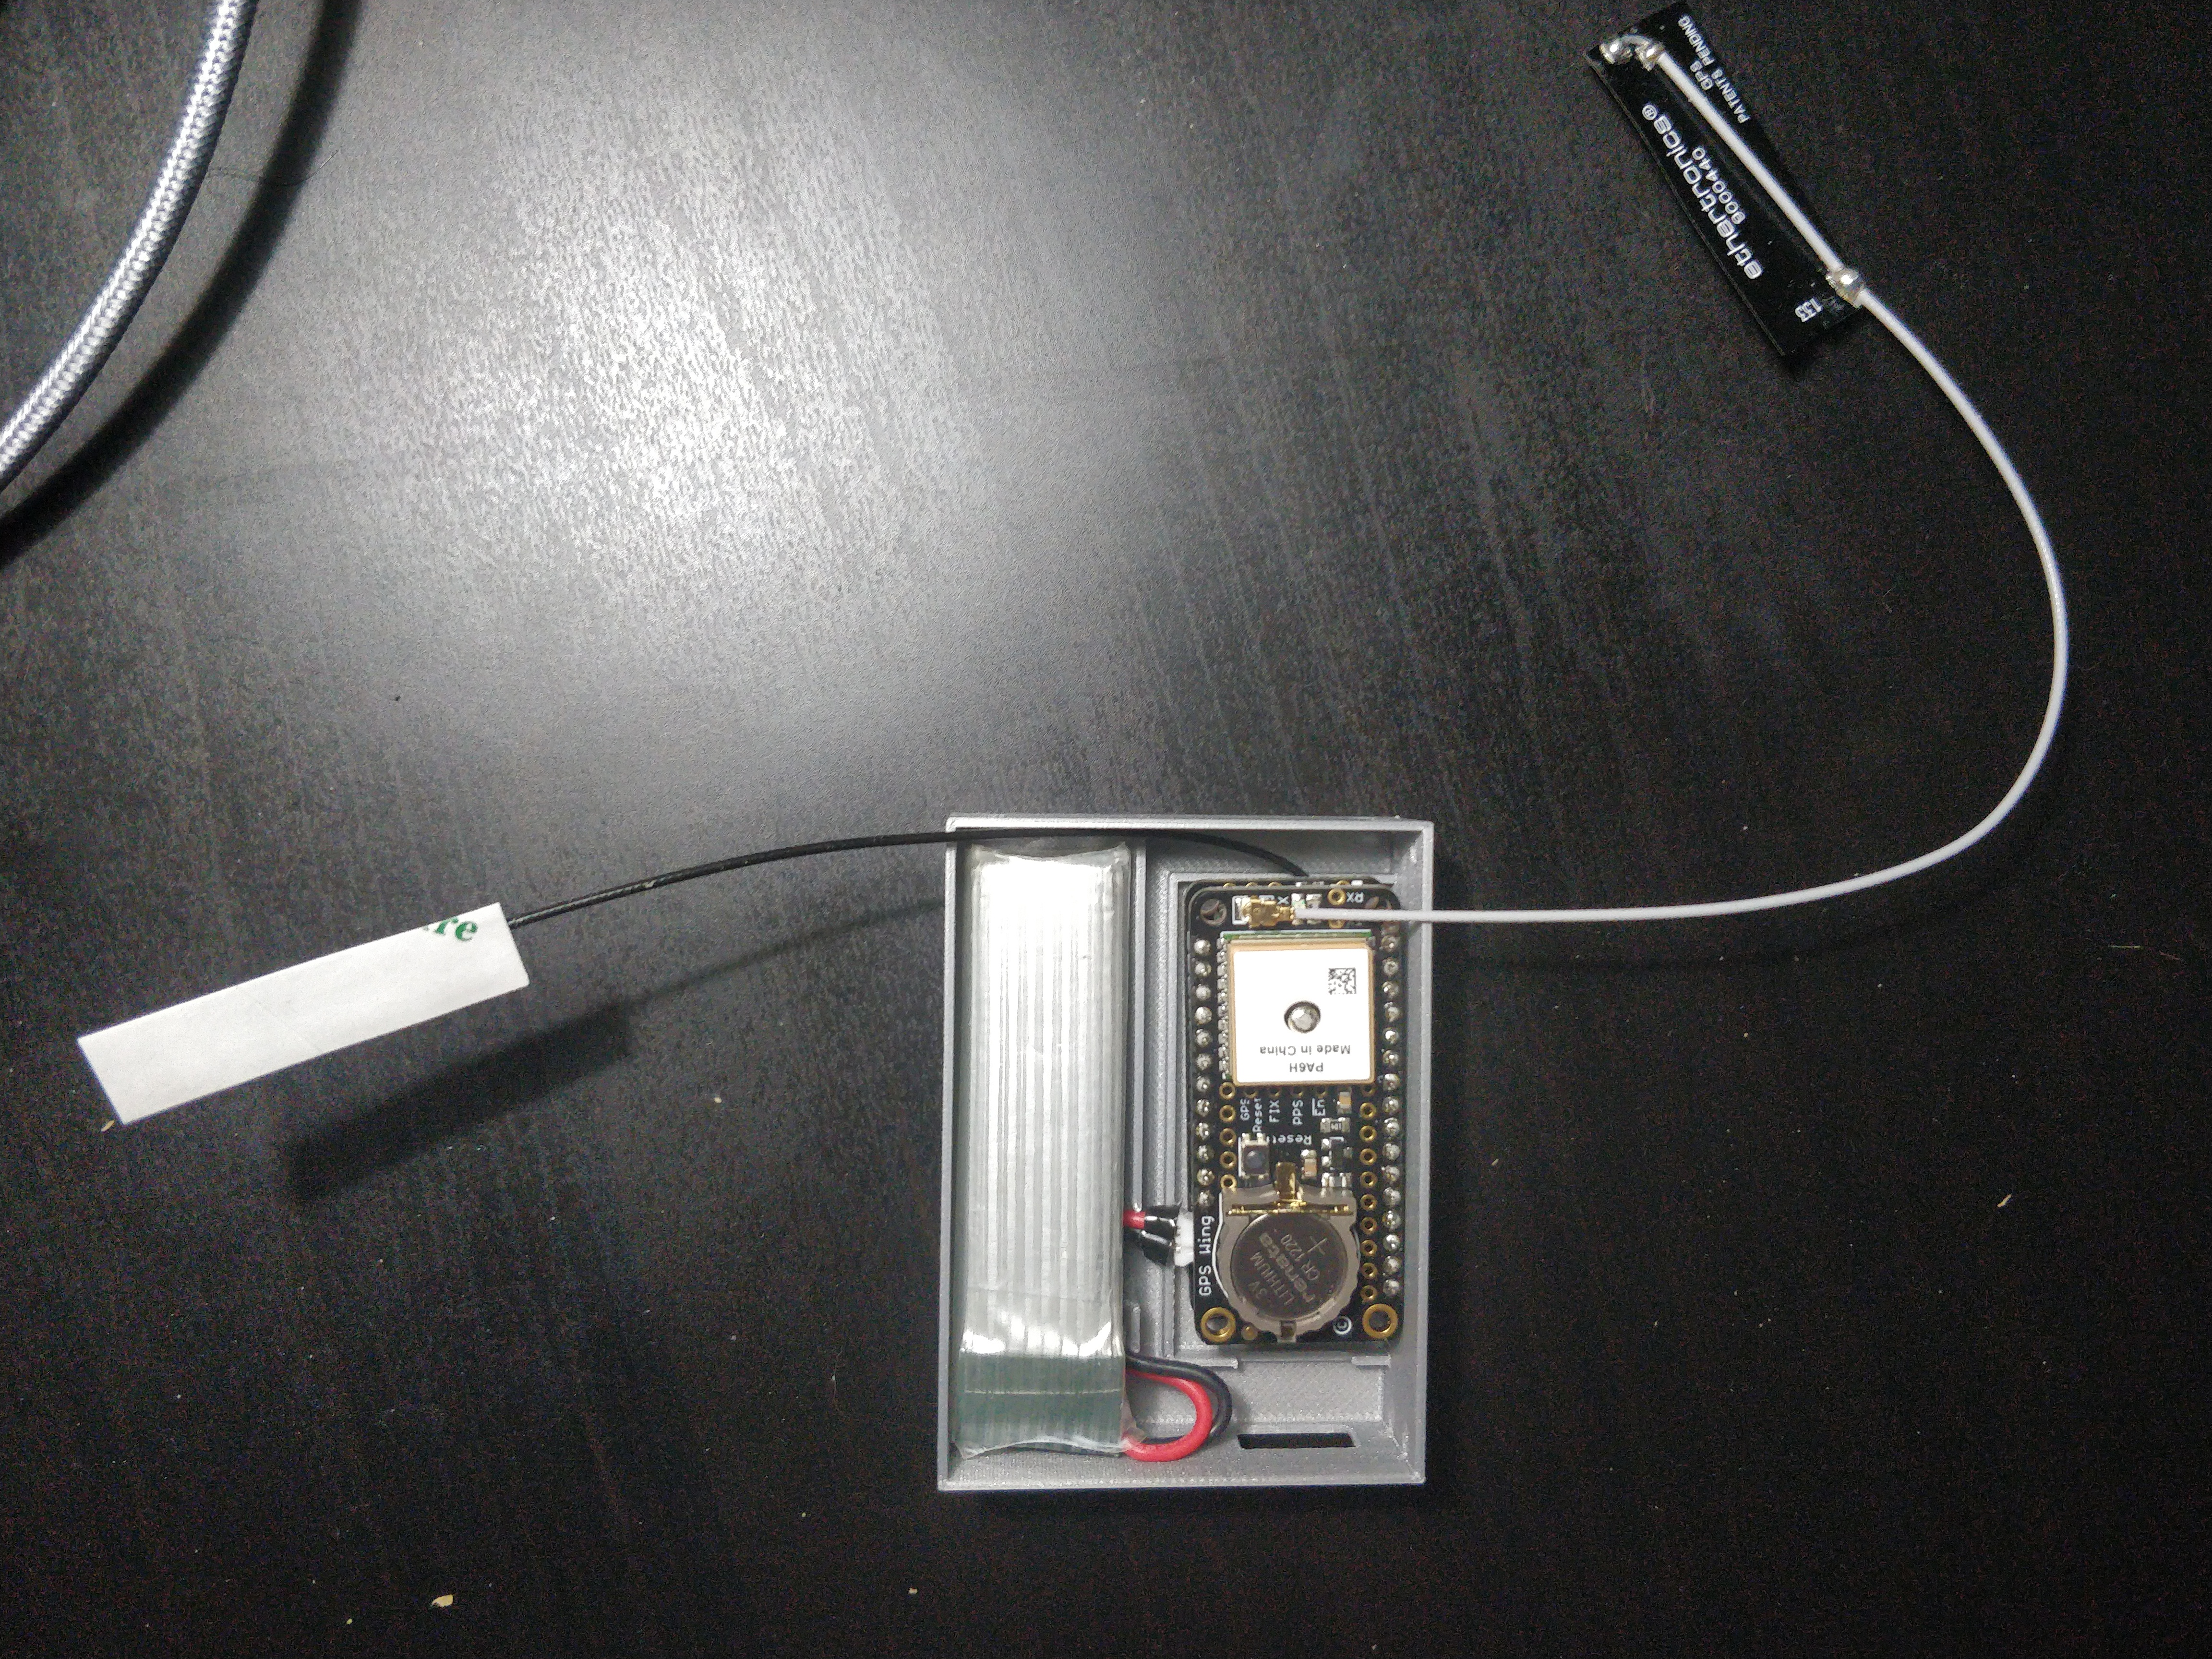
\includegraphics[angle=90,width=\textwidth]{../figures/Pics/secondcase1.jpg}
            \vspace{5pt}
            \caption{Case with antennae}            
            \label{fig:case2antennasplay}
        \end{subfigure}
        \hfill
        \begin{subfigure}[b]{0.3\textwidth}  
            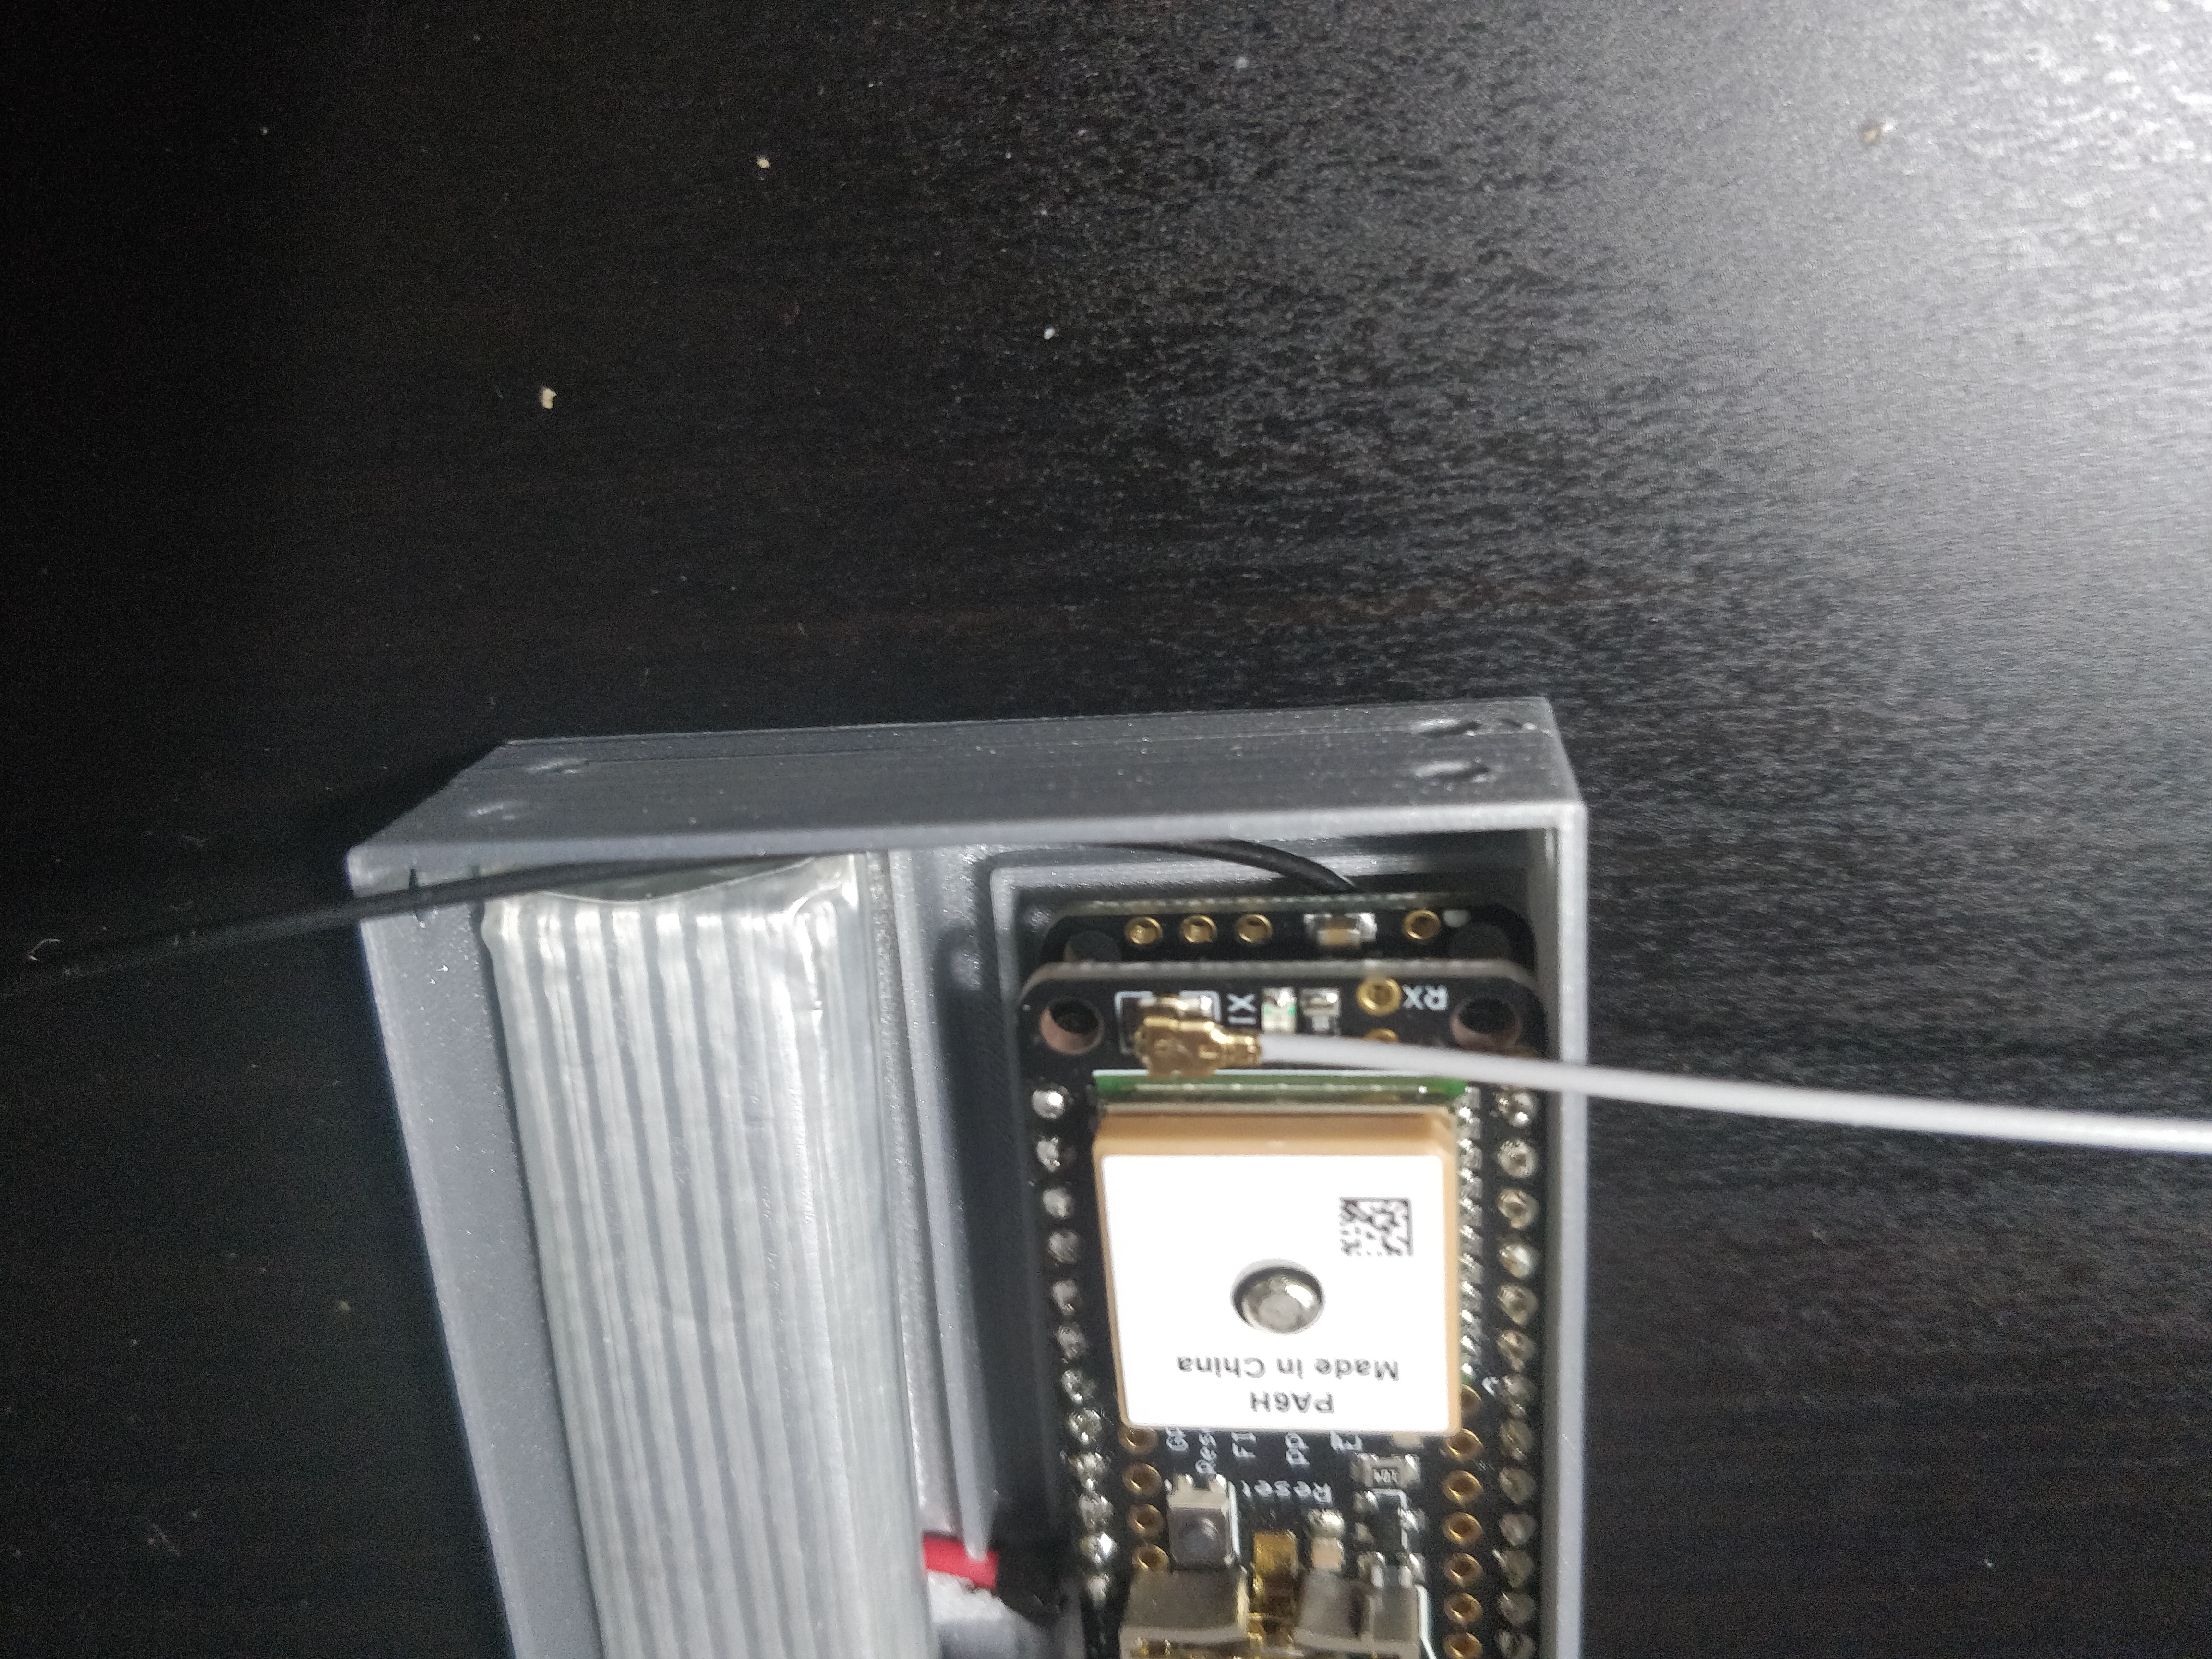
\includegraphics[angle=90,width=\textwidth]{../figures/Pics/secondcase2.jpg}
            \vspace{5pt}
            \caption{Antenna raising issue}                    
            \label{fig:case2antennaissue}
        \end{subfigure}
        \hspace*{\fill}
        \vskip\baselineskip
        \hspace*{\fill}
        \begin{subfigure}[b]{0.3\textwidth}   
            \captionsetup{justification=centering}
            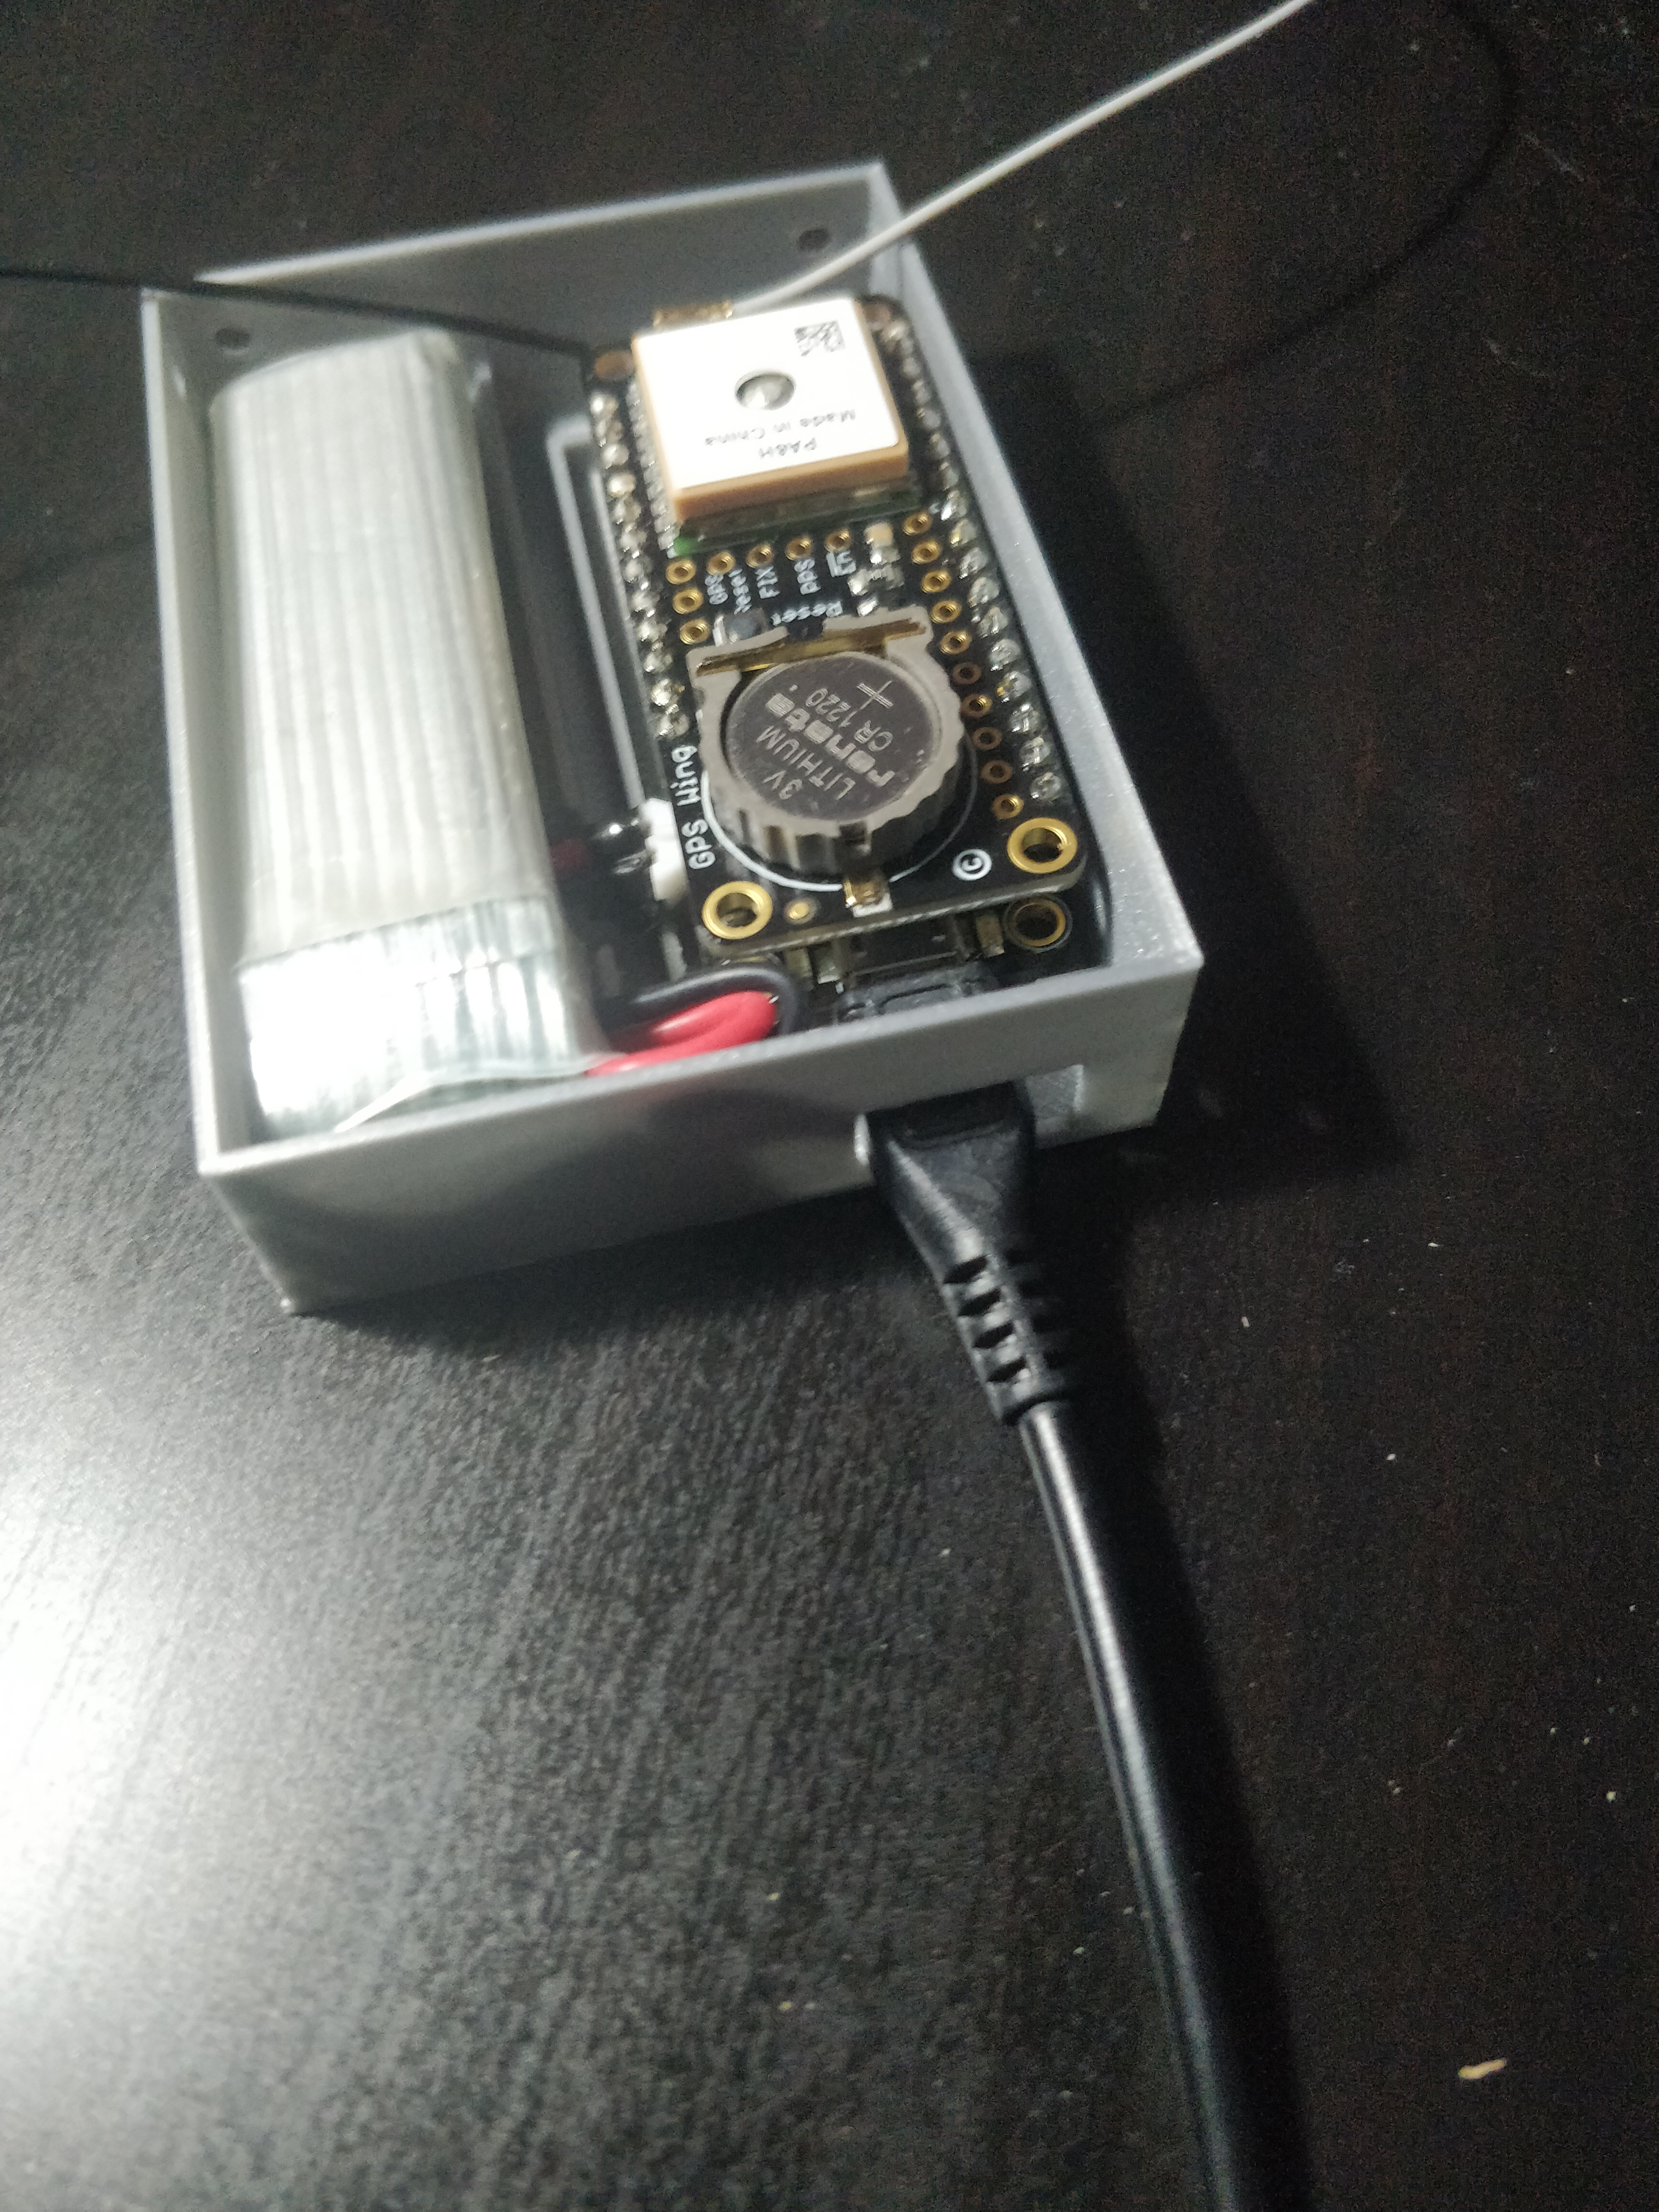
\includegraphics[width=\textwidth]{../figures/Pics/secondcase3.jpg}
            \vspace{1pt}
            \caption{Angled front view with \acrshort{usb} connection}
        \end{subfigure}
        \hfill
        \begin{subfigure}[b]{0.3\textwidth}           
            \captionsetup{justification=centering}
            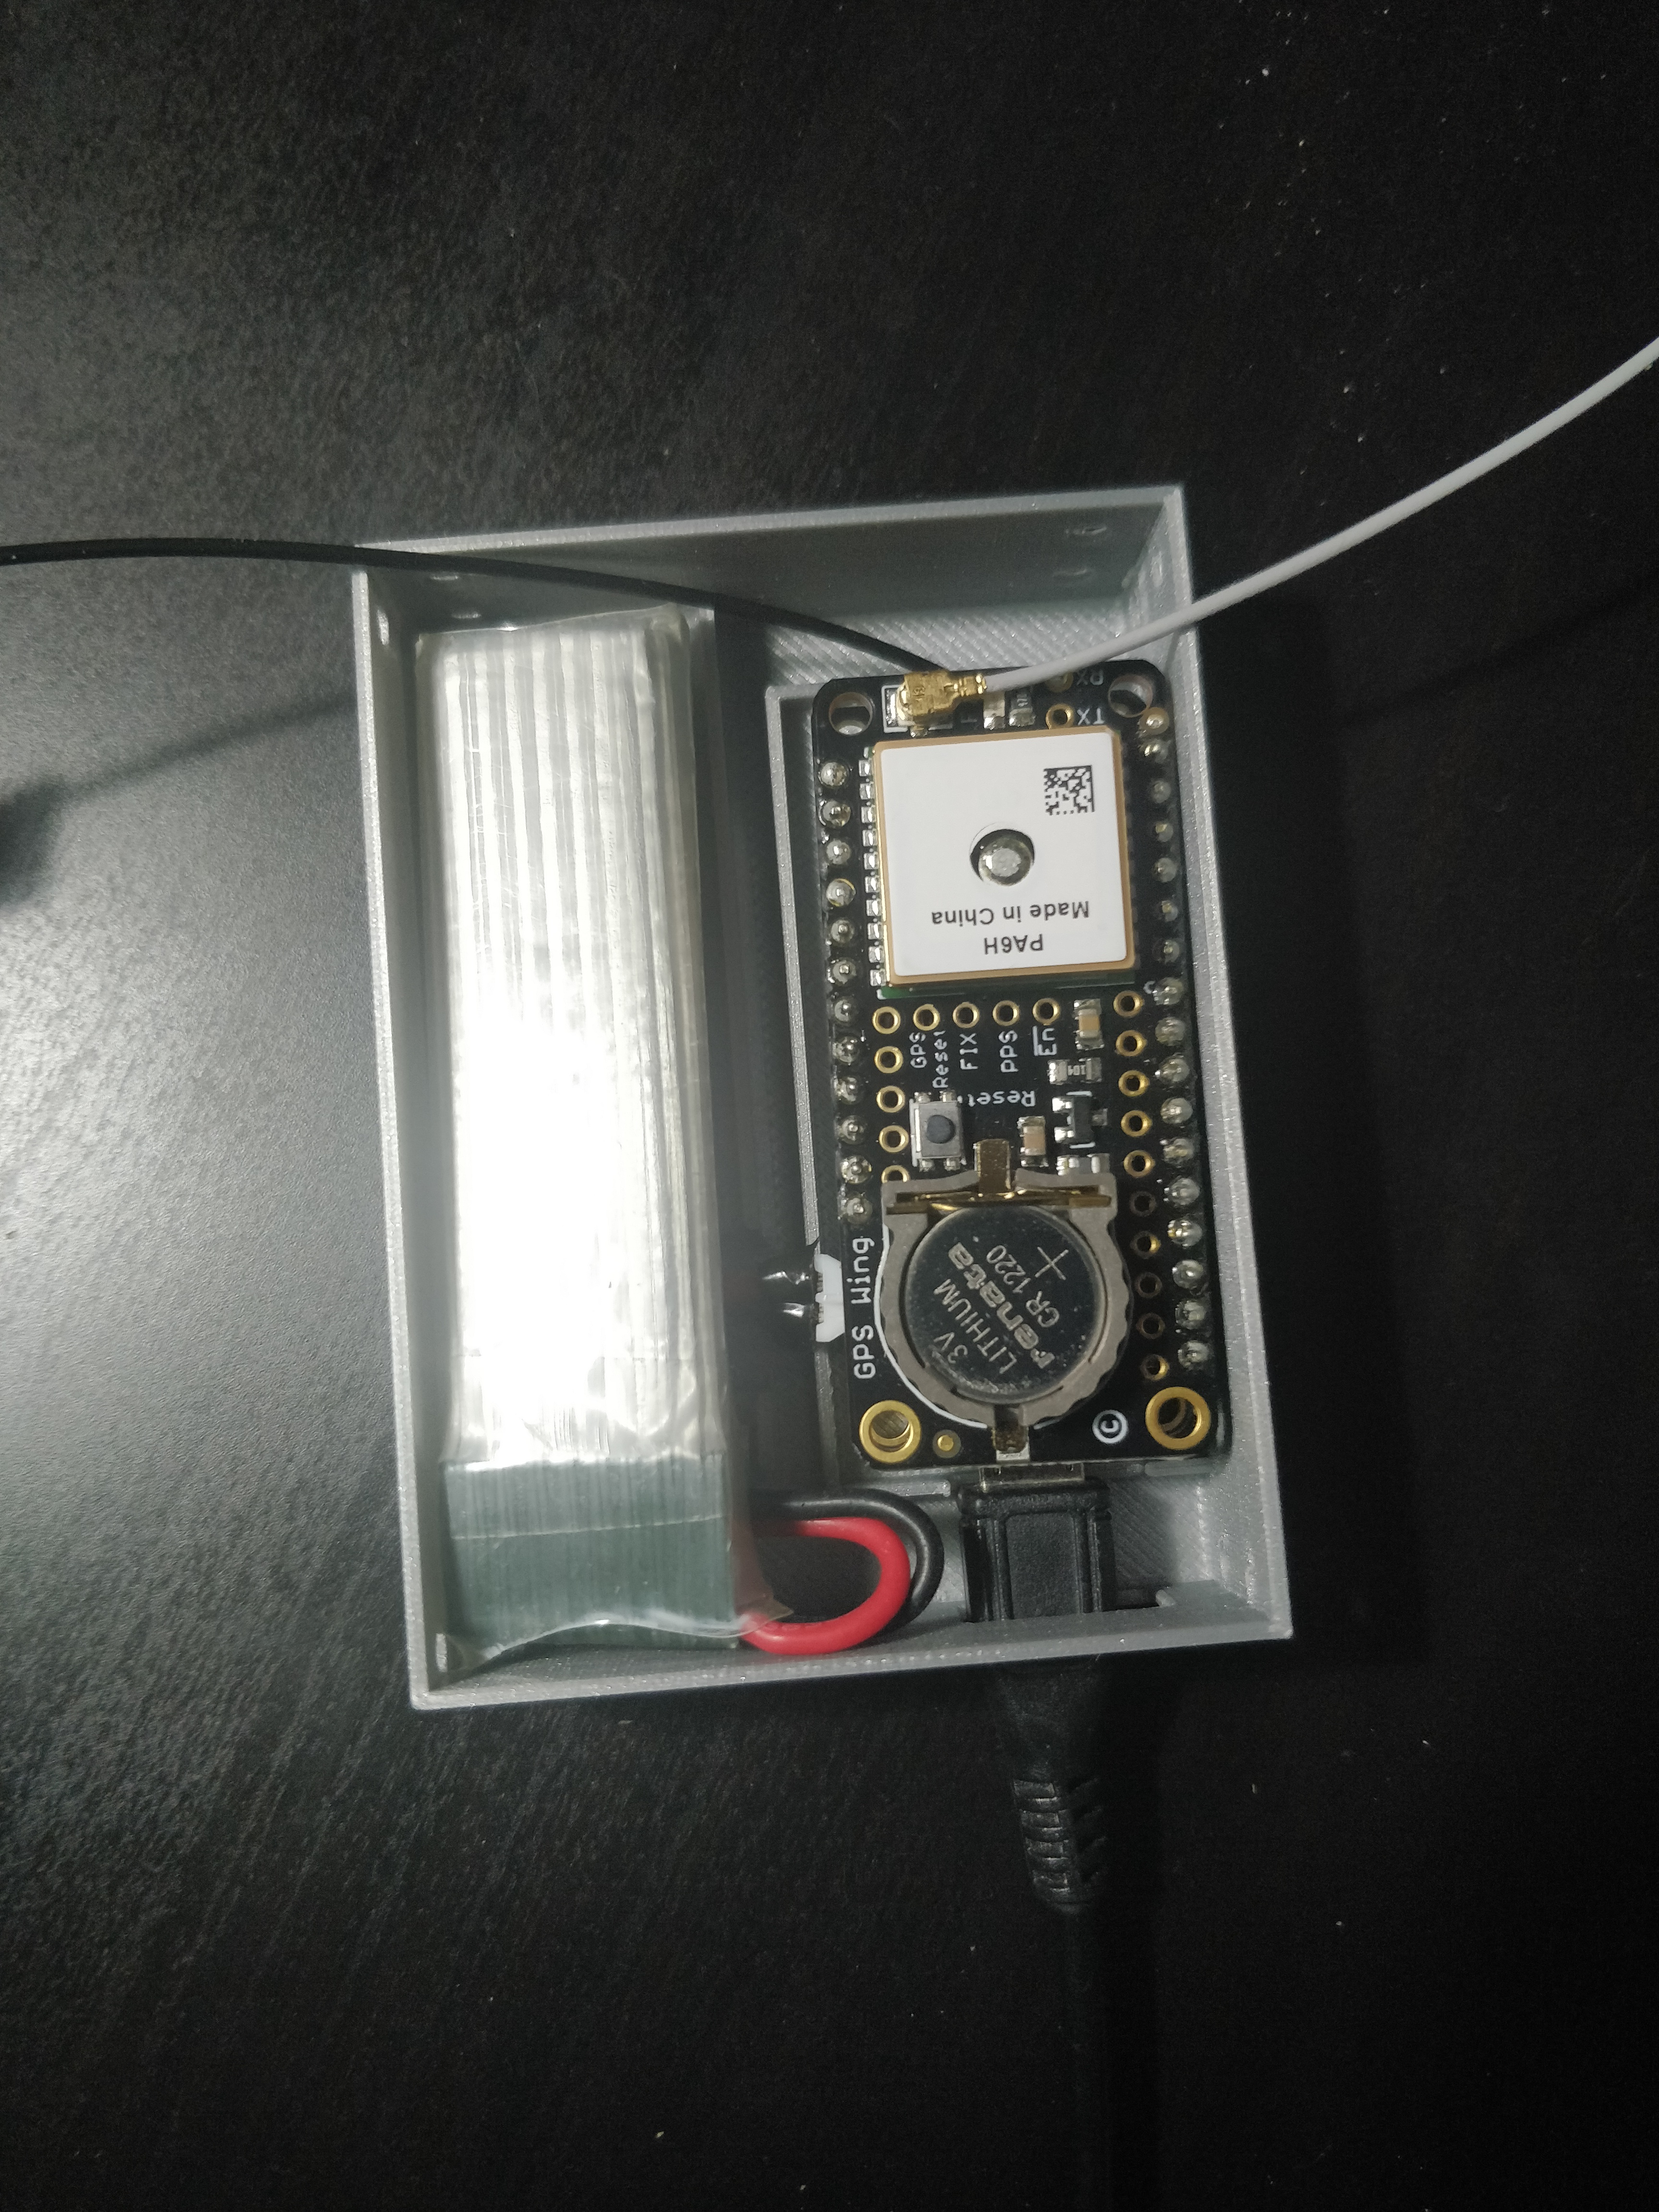
\includegraphics[width=\textwidth]{../figures/Pics/secondcase4.jpg}
            \vspace{5pt}
            \caption{Top view with \acrshort{usb} connection}
        \end{subfigure}
        \hspace*{\fill}
    \end{figure}
    \vfill
    \clearpage

    % \begin{figure}[H]        
    %     \label{case2dwg}
    %     \caption{Case 2 dimensional drawing}
    %     \includegraphics[angle=-90,width=\textwidth]{../../Design/case2.pdf}
    % \end{figure}   

    % \begin{figure}[H]        
        % \includepdf[pagecommand={},angle=-90,scale=0.9,pagecommand=\section{Case 2 dimensional drawing \label{fig:case2dwg}}]{../../Design/case2.pdf}
        % \label{fig:case2dwg}
    % \end{figure}
    % \clearpage

    \begin{figure}[H]      
        \caption{Case 2 dimensional drawings}
        \includepdf[pagecommand={},angle=-90,scale=0.9]{../../Design/case2.pdf}  
        \label{fig:case2dwg}
    \end{figure}
   


\begin{landscape}

\chapter{Purchasing lists}

    \begin{xltabular}{\linewidth}{|cYccccc|}
        \caption{Preliminary hardware list} \label{table:prelimhardwarelist} \\
        \hline

        \rowcolor{tableh2}
        Part & Description & Quantity  & Price per unit & Supplier & SKU & Web link \\
        \endfirsthead

        \caption{Preliminary hardware list (cont.)}\\
        \hline
        \rowcolor{tableh2}
        Part & Description & Quantity  & Price per unit & Supplier & SKU & Web link \\
        \endhead
        \endfoot

        \hline
        \rowcolor{tableh1}
        \multicolumn{7}{|c|}{Common requirement} \\
        \hline
        SX1262 LoRa HAT & LoRa radio for the Raspberry Pi & 1   & 28.10 & PiHut & WAV-16806 & \href{https://thepihut.com/products/sx1262-lora-hat-for-raspberry-pi-868mhz-for-europe-asia-africa}{Link \faExternalLink} \\
        \hline
        500mAh LiPo battery	& &	1 &	6.00	& PiHut &	105189 &	\href{https://thepihut.com/products/500mah-3-7v-lipo-battery}{Link \faExternalLink} \\
        \hline
        \rowcolor{tableh1}
        \multicolumn{7}{|c|}{Transmitter Set 1} \\
        \hline
        Challenger RP2040 &	microcontroller with lora radio	& 1 &	21.5	& PiHut	& 104944	& \href{https://thepihut.com/products/challenger-rp2040-lora-868mhz}{Link \faExternalLink} \\
        \hline
        GPS Featherwing &	gps module (uart)	& 1 &	24.6 &	PiHut &	ADA3133 &	\href{https://thepihut.com/products/adafruit-ultimate-gps-featherwing}{Link \faExternalLink} \\
        \hline
        \rowcolor{tableh1}
        \multicolumn{7}{|c|}{Transmitter Set 2 - I\textsuperscript{2}C alternative} \\
        \hline
        Feather RP2040 &	microcontroller	& 1	& 11.4	& PiHut &	ADA4884	& \href{https://thepihut.com/products/adafruit-feather-rp2040}{Link \faExternalLink} \\
        \hline
        LoRa Featherwing &	lora radio (i2c) &	1	& 19.5 &	PiHut &	ADA3231 &	\href{https://thepihut.com/products/adafruit-lora-radio-featherwing-rfm95w-900-mhz}{Link \faExternalLink} \\
        \hline
        GPS breakout &	gps module (i2c) &	1 &	29.7 &	PiHut &	PIM525 &	\href{https://thepihut.com/products/pa1010d-gps-breakout}{Link \faExternalLink} \\
        \hline
        uFL connector &	to get an antenna onto the lora board &	5	& 0.8 &	PiHut	& ADA1661 &	\href{https://thepihut.com/products/ufl-smt-antenna-connector}{Link \faExternalLink} \\
        \hline
        \rowcolor{tableh1}
        \multicolumn{7}{|c|}{Antenna Options} \\
        \hline
        W3013 & 	ceramic  & 	2 & 	1.48 & 	Mouser & 	673-W3013	 & \href{https://www.mouser.co.uk/ProductDetail/Pulse-Electronics/W3013?qs=sk8jCzc\%252BkzSRDEaf6KYAUA\%3D\%3D}{Link \faExternalLink} \\
        \hline
        PIOV008NRAA-100	 & strip with ufl &  	1 & 	1.87 & 	Mouser & 	523-PIOV008NRAA-100	 & \href{https://www.mouser.co.uk/ProductDetail/Amphenol-MCP/PIOV008NRAA-100?qs=GedFDFLaBXFCaCiGvxFhnA\%3D\%3D}{Link \faExternalLink} \\
        \hline
        318020612 & 	Outdoor antenna - N male	 & 1	 & 30.8 & 	Mouser & 	713-318020612 & 	\href{https://www.mouser.co.uk/ProductDetail/Seeed-Studio/318020612?qs=TuK3vfAjtkUc5jgrDpnp\%252Bw\%3D\%3D}{Link \faExternalLink} \\
        \hline
        &   amazon option with included cable and adapter	 & 1	 & 30.99 & 	Amazon	 & &	\href{https://amzn.eu/d/daYwpxw}{Link \faExternalLink} \\
        \hline
        CAB.951	 & N female - SMA male, 1m	 & 1	 & 17.13 & 	Mouser & 	960-CAB.951	 & \href{https://www.mouser.co.uk/ProductDetail/Taoglas/CAB.951?qs=RuW\%2Fu\%252BNMQmvLr59ScsVBcw\%3D\%3D}{Link \faExternalLink} \\
        \hline
        &  much cheaper amazon option & 	1 & 	11.98	 & Amazon	 & &	\href{https://amzn.eu/d/d8hsE0k}{Link \faExternalLink} \\
        \hline
        Pigtail Antenna	 & only if none of the other options work & 	2	 & 4.9 & 	PiHut & 	105078	 & \href{https://thepihut.com/products/lora-antenna-with-pigtail-868mhz-black}{Link \faExternalLink} \\
        \hline
        Raspberry Pi & 	it's okay I actually own a Pi3 & 	1	 & 219.99	 & Amazon	& & 	\href{https://amzn.eu/d/7W5NpuZ}{Link \faExternalLink} \\
        \hline
    \end{xltabular}

    \begin{xltabular}{\linewidth}{|cYccccc|}
        \caption{Updated hardware list} \label{table:updatedhardwarelist}\\
        \hline
        \rowcolor{tableh2}
        Part & Description & Quantity  & Price per unit & Supplier & SKU & Web link \\
        \endfirsthead

        \caption{Updated hardware list (cont.)}\\
        \hline
        \rowcolor{tableh2}
        Part & Description & Quantity  & Price per unit & Supplier & SKU & Web link \\
        \endhead
        \endfoot

        \hline
        \rowcolor{tableh1}
        \multicolumn{7}{|c|}{Transmitter} \\
        \hline
        3178	 & Feather M0 LoRa & 1 & 	30.76 & 	 Mouser & 	485-3178 & 	\href{https://www.mouser.co.uk/ProductDetail/Adafruit/3178?qs=TlVEbN\%2FgKDkhUZkXCJivzw\%3D\%3D}{Link \faExternalLink} \\
        \hline
        3133	 & GPS Featherwing	 & 1	 & 21.96	  & 	Mouser & 	485-3133 & 	\href{https://www.mouser.co.uk/ProductDetail/Adafruit/3133?qs=TlVEbN\%2FgKDmpiId5nasRCA\%3D\%3D}{Link \faExternalLink} \\
        \hline
        & Pimoroni equivalent & 	1	 & 24.6		 & Pimoroni & 	ADA3133 & 	\href{https://shop.pimoroni.com/products/adafruit-ultimate-gps-featherwing?variant=21438274887}{Link \faExternalLink} \\
        \hline

        \rowcolor{tableh1}
        \multicolumn{7}{|c|}{Receiver} \\
        \hline
        3231	 & LoRa Featherwing & 	1	 & 18.68	 & 	Digikey	 & 1528-1741-ND	 & \href{https://www.digikey.co.uk/en/products/detail/adafruit-industries-llc/3231/6193593}{Link \faExternalLink} \\
        \hline
        & Equivalent	 & 1	 & 19.5	 & 	Pimoroni	 & ADA3231 & 	\href{https://shop.pimoroni.com/products/adafruit-lora-radio-featherwing-rfm95w-900-mhz-radiofruit?variant=2089110306826}{Link \faExternalLink} \\
        \hline
        & Bonnet OLED alternative	 & 1	 & 31.8		 & Pimoroni & 	ADA4074	 & \href{https://shop.pimoroni.com/products/adafruit-lora-radio-bonnet-with-oled-rfm95w-915mhz-radiofruit?variant=27912635220051}{Link \faExternalLink} \\
        \hline
        & + headers & 	1 & 	2.1	 & 	Pimoroni	 & COM0003 & 	\href{https://shop.pimoroni.com/products/booster-header?variant=47414520906}{Link \faExternalLink} \\
        \hline

        \rowcolor{tableh1}
        \multicolumn{7}{|c|}{Accessories} \\
        \hline
        2258	 & Pi Case & 	1 & 	7	 & 	Mouser	 & 485-2258	 & \href{https://www.mouser.co.uk/ProductDetail/Adafruit/2258?qs=GURawfaeGuAHsbLMi7envw\%3D\%3D}{Link \faExternalLink} \\
        \hline
        &  Equivalent	 & 1	 & 7.8	 & 	Pimoroni	 & ADA2258	 & \href{https://shop.pimoroni.com/products/adafruit-raspberry-pi-b-case-smoke-base-w-clear-top?variant=1005886429}{Link \faExternalLink} \\
        \hline
        4410	 & lipo (jst) charger	 & 1 & 	5.24	 & Mouser	 & 485-4410 & 	\href{https://www.mouser.co.uk/ProductDetail/Adafruit/4410?qs=wnTfsH77Xs5n1kx9qVo63A\%3D\%3D}{Link \faExternalLink} \\
        \hline
        2830 & 	stacking headers 1st level & 	1 & 		1.1	 & Mouser	 & 485-2830 & 	\href{https://www.mouser.co.uk/ProductDetail/Adafruit/2830?qs=xE9dPqTLfL4XzxEZXTz\%252BEA\%3D\%3D}{Link \faExternalLink} \\
        \hline
        & Equivalent	 & 1	 & 1.1	 & 	Pimoroni	 & ADA2830	 & \href{https://shop.pimoroni.com/products/feather-stacking-headers-12-pin-and-16-pin-female-headers?variant=13709873863}{Link \faExternalLink} \\
        \hline
        2886	 & stacking headers base	 & 1	 & 0.836	 & 	Mouser & 	485-2886 & 	\href{https://www.mouser.co.uk/ProductDetail/Adafruit/2886?qs=xE9dPqTLfL61eEvyw283TQ\%3D\%3D}{Link \faExternalLink} \\
        \hline
        &   Equivalent	 & 1	 & 1.2	 & 	Pimoroni & 	ADA2886	 & \href{https://shop.pimoroni.com/products/feather-header-kit-12-pin-and-16-pin-female-header-set?variant=13710014791}{Link \faExternalLink} \\
        \hline

        \rowcolor{tableh1}
        \multicolumn{7}{|c|}{Battery} \\
        \hline
        4714 & 	JST PH Female jumper	 & 1 & 	0.836 & 		Mouser & 	485-4714 & 	\href{https://www.mouser.co.uk/ProductDetail/Adafruit/4714?qs=hd1VzrDQEGi2qAbAJE0pRQ\%3D\%3D}{Link \faExternalLink} \\
        \hline
        RS PRO battery	 & LiPo 1.8Ah	 & 1	 & 10.86	 & RS & 	144-9405 & 	\href{https://uk.rs-online.com/web/p/speciality-size-rechargeable-batteries/1449405}{Link \faExternalLink} \\
        \hline
        Alternative  & 1.2mAh, doesn't require jumper or housing 	 & 1	 & 9.9	 & 	Pimoroni & 	BAT00044	 & \href{https://shop.pimoroni.com/products/lipo-battery-pack?variant=20429082183}{Link \faExternalLink} \\
        \hline
        PHR-2	 & JST PH Female connector housing	 & 1	 & 0.66	 & RS	 & 820-1466 & 	\href{https://uk.rs-online.com/web/p/wire-housings-plugs/8201466}{Link \faExternalLink} \\
        \hline

        \rowcolor{tableh1}
        \multicolumn{7}{|c|}{Antenna} \\
        \hline
        ANT-868-CPA	 & ceramic 	 & 1	 & 2.97	  & Mouser	 & 712-ANT-868-CPA & 	\href{https://www.mouser.co.uk/ProductDetail/Linx-Technologies/ANT-868-CPA?qs=wnTfsH77Xs69O4Svqy49rA\%3D\%3D}{Link \faExternalLink} \\
        \hline
        PIOV008NRAA-100	 & strip with ufl  & 	1	 & 1.87	 & Mouser	 & 523-PIOV008NRAA-100 & 	\href{https://www.mouser.co.uk/ProductDetail/Amphenol-MCP/PIOV008NRAA-100?qs=GedFDFLaBXFCaCiGvxFhnA\%3D\%3D}{Link \faExternalLink} \\
        \hline
        318020612 & 	Outdoor antenna - N male	 & 1	 & 30.8 & 	Mouser	 & 713-318020612	 & \href{https://www.mouser.co.uk/ProductDetail/Seeed-Studio/318020612?qs=TuK3vfAjtkUc5jgrDpnp\%252Bw\%3D\%3D}{Link \faExternalLink} \\
        \hline
        CAB.951	 & N female - SMA male, 1m	 & 1	 & 17.13 & 	Mouser	 & 960-CAB.951	 & \href{https://www.mouser.co.uk/ProductDetail/Taoglas/CAB.951?qs=RuW\%2Fu\%252BNMQmvLr59ScsVBcw\%3D\%3D}{Link \faExternalLink} \\
        \hline
        CONUFL001-SMD-T	 & uFL connector	 & 5	 & 0.625	 & 	Mouser	 & 712-CONUFL001-SMD-T & 	\href{https://www.mouser.co.uk/ProductDetail/Linx-Technologies/CONUFL001-SMD-T?qs=EU6FO9ffTwfRdkBeQTdJWQ\%3D\%3D}{Link \faExternalLink} \\
        \hline
        CASMA-UFL-1	 & uFL to SMA F	 & 2	 & 8.71	 & Mouser	 & 125-CASMA-UFL-1	 & \href{https://www.mouser.co.uk/ProductDetail/MultiTech/CASMA-UFL-1?qs=7MVldsJ5UawLWQzcvLUp6A\%3D\%3D}{Link \faExternalLink} \\
        \hline
        & Equivalent	 & 2	 & 3.9	 & 	Pimoroni	 & ADA851	 & \href{https://shop.pimoroni.com/products/adafruit-sma-to-ufl-u-fl-ipx-ipex-rf-adapter-cable?variant=433911117}{Link \faExternalLink} \\
        \hline

        \rowcolor{tableh1}
        \multicolumn{7}{|c|}{Additional Antennae} \\
        \hline
        W3214	 & ceramic  & 	1 & 	2.08	 & 	Mouser	 & 673-W3214 & 	\href{https://www.mouser.co.uk/ProductDetail/Pulse-Electronics/W3214?qs=l7cgNqFNU1gaMT1NL8sSIA\%3D\%3D}{Link \faExternalLink} \\
        \hline
        M620720 & 	ceramic  & 	1	 & 1.73	 & 	Mouser & 	581-M620720 & 	\href{https://www.mouser.co.uk/ProductDetail/Ethertronics-KYOCERA-AVX/M620720?qs=MLItCLRbWsxW2ijaVr6ojw\%3D\%3D}{Link \faExternalLink} \\
        \hline
        W3013	 & ceramic 	 & 1	 & 1.48	 & 	Mouser	 & 673-W3013 & 	\href{https://www.mouser.co.uk/ProductDetail/Pulse-Electronics/W3013?qs=sk8jCzc\%252BkzSRDEaf6KYAUA\%3D\%3D}{Link \faExternalLink} \\
        \hline

    \end{xltabular}

    \begin{xltabular}{\linewidth}{|Ycccccc|}
        \caption{Antennae list} \label{table:antennaelist} \\
        \hline

        \rowcolor{tableh2}
        Description & Part & Name  & Price & Supplier & SKU & Web link \\
        \endfirsthead

        \caption{Preliminary hardware list (cont.)}\\
        \hline
        \rowcolor{tableh2}
        Part & Description & Quantity  & Price per unit & Supplier & SKU & Web link \\
        \endhead
        \endfoot

        \hline
        Original antenna: & 	318020612 & 	Outdoor antenna - N male & 	30.8 & 	Mouser	 & 713-318020612 & 	\href{https://www.mouser.co.uk/ProductDetail/Seeed-Studio/318020612?qs=TuK3vfAjtkUc5jgrDpnp\%252Bw\%3D\%3D}{Link \faExternalLink} \\
        \hline
        Suggested replacement:	 & 318020690	 & 5.8dBi antenna & 	41.24 & 	Farnell	 & 4060414 & 	\href{https://uk.farnell.com/seeed-studio/318020690/antenna-fiberglass-863-to-870mhz/dp/4060414}{Link \faExternalLink} \\
        \hline
        Cheaper alternative:	 & 318020708	 & 3dBi antenna	 & 24.72	 & Farnell	 & 4060419 & 	\href{https://uk.farnell.com/seeed-studio/318020708/antenna-fiberglass-860-to-930mhz/dp/4060419}{Link \faExternalLink} \\
        \hline
        Lora antenna	 & 211140-0100	 & 0.3dBi at 868, 38mm	 & 1.7	 & Farnell	 & 3498957 & 	\href{https://uk.farnell.com/molex/211140-0100/ism-antenna-902-928mhz-1dbi/dp/3498957?st=ism\%20antenna}{Link \faExternalLink} \\
        \hline
        Additional lora antenna	 & 1002289F0-AA10L0200 & 	1.8 dBi & 	3.95 & 	Farnell	 & 3407000 & 	\href{https://uk.farnell.com/avx/1002289f0-aa10l0200/fpc-embedded-antenna-2-69ghz-4/dp/3407000}{Link \faExternalLink} \\
        \hline
        gps antenna	 & 9000440	 &  & 	1.79	 & Farnell & 	3407009 & 	\href{https://uk.farnell.com/avx/9000440/pcb-antenna-1-593-1-61ghz-2-5dbi/dp/3407009}{Link \faExternalLink} \\
        \hline
        additional gps antenna if within budget	 & APKD1507G2-0100S	 & 	 & 6.83 & 	Farnell	 & 3924367 & 	\href{https://uk.farnell.com/abracon/apkd1507g2-0100s/patch-antenna-1-60538-1-59806ghz/dp/3924367}{Link \faExternalLink} \\
        \hline
        alternative selected lora	 & 206764-0100	  & & 	3.31	 & Farnell	 & 2885764	 & \href{https://uk.farnell.com/molex/206764-0100/omni-antenna-lin-902-928mhz-1/dp/2885764?st=ism\%20antenna}{Link \faExternalLink} \\
        \hline
    \end{xltabular}


\chapter{Data}

    \section{Power Consumption}
    \begin{table}[H]
        \centering
        \caption{Power meter recordings}
        \begin{tabular}{|cc|}
            \hline
            Timestamp        & Consumption (mAh) \\
            \hline
            21/01/2023 19:46 & 0                 \\
            21/01/2023 22:43 & 1                 \\
            22/01/2023 13:40 & 8                 \\
            22/01/2023 16:58 & 10                \\
            22/01/2023 18:38 & 11                \\
            22/01/2023 21:31 & 12                \\
            22/01/2023 22:26 & 13                \\
            23/01/2023 11:00 & 19                \\
            23/01/2023 14:40 & 21                \\
            23/01/2023 19:39 & 23                \\
            \hline
        \end{tabular}
        \label{table:powermeter}
    \end{table}

    \begin{table}[H]
        \centering
        \caption{Discharge data sample - 230213.csv}
        \begin{xltabular}{\linewidth}{|cccccccc|}
            \hline
            Timestamp & Datetime & Packet & Longitude & Latitude & Altitude & Fix & Voltage \\
            \hline
            1676326772.56411 & 13-02-23 22:19:32 & 11 & 5223.\censor{6768} & 133.\censor{2758} & 87.10 & 0 & 4.183 \\
            1676326777.5640159 & 13-02-23 22:19:37 & 12 & 5223.\censor{6821} & 133.\censor{2824} & 87.10 & 1 & 4.183 \\
            1676326782.5647342 & 13-02-23 22:19:42 & 12 & 5223.\censor{6821} & 133.\censor{2824} & 87.10 & 0 & 4.189 \\
            1676326787.564926 & 13-02-23 22:19:47 & 12 & 5223.\censor{6821} & 133.\censor{2824} & 87.10 & 0 & 4.183 \\
            \multicolumn{8}{|c|}{$\cdots$} \\
            1676380803.0929441 & 14-02-23 13:20:03 & 10188 & 5223.\censor{6680} & 133.\censor{2785} & 69.10 & 0 & 3.564 \\
            1676380808.0946279 & 14-02-23 13:20:08 & 10188 & 5223.\censor{6680} & 133.\censor{2785} & 69.10 & 0 & 3.557 \\
            1676380813.0988088 & 14-02-23 13:20:13 & 10188 & 5223.\censor{6680} & 133.\censor{2785} & 69.10 & 0 & 3.564 \\
            1676380818.1010823 & 14-02-23 13:20:18 & 10188 & 5223.\censor{6680} & 133.\censor{2785} & 69.10 & 0 & 3.564 \\
            \hline
        \end{xltabular}
        \label{table:dischargedata}
    \end{table}

    \begin{table}[H]
        \centering
        \caption{Charge data sample - 230214.csv}
        \begin{xltabular}{\linewidth}{|cccccccc|}
            \hline
            Timestamp & Datetime & Packet & Longitude & Latitude & Altitude & Fix & Voltage \\
            \hline
            1676392659.3032475 & 14-02-23 16:37:39 & 0 & 0.0000 & 0.0000 & 0.00 & 0 & 1.617 \\
            1676392664.3044226 & 14-02-23 16:37:44 & 0 & 0.0000 & 0.0000 & 0.00 & 0 & 1.695 \\
            1676392669.3057065 & 14-02-23 16:37:49 & 0 & 0.0000 & 0.0000 & 0.00 & 0 & 1.772 \\
            1676392674.305263 & 14-02-23 16:37:54 & 0 & 0.0000 & 0.0000 & 0.00 & 0 & 1.830 \\
            \multicolumn{8}{|c|}{$\cdots$} \\
            1676428057.1960237 & 15-02-23 02:27:37 & 6260 & 5223.\censor{6670} & 133.\censor{2817} & 87.50 & 1 & 4.131 \\
            1676428062.1964362 & 15-02-23 02:27:42 & 6261 & 5223.\censor{6670} & 133.\censor{2817} & 87.50 & 1 & 4.131 \\
            1676428067.197315 & 15-02-23 02:27:47 & 6262 & 5223.\censor{6665} & 133.\censor{2818} & 87.60 & 1 & 4.131 \\
            1676428072.1974156 & 15-02-23 02:27:52 & 6263 & 5223.\censor{6665} & 133.\censor{2813} & 87.60 & 1 & 4.137 \\
            \hline
        \end{xltabular}
        \label{table:chargedata}
    \end{table}
    \clearpage

    \section{Distance}

    \begin{lstlisting}[language=XML,caption={Distance Test 1 sample - 2023-02-17\_17\_Feb\_2023\_1\_41\_52\_pm.kml},label=kmltest1]
    <gx:MultiTrack>
        <altitudeMode>absolute</altitudeMode>
        <gx:interpolate>0</gx:interpolate>
        <gx:Track>
          <gx:coord>-1.56132623 52.38261212 62.51</gx:coord>
          <when>2023-02-17T13:44:48Z</when>
          <gx:coord>-1.56123128 52.38268469 127.56</gx:coord>
          <when>2023-02-17T13:45:10Z</when>
          <gx:coord>-1.56129532 52.38279329 126.44</gx:coord>
          <when>2023-02-17T13:45:14Z</when>
          <gx:coord>-1.56138629 52.38286398 127.49</gx:coord>
          <when>2023-02-17T13:45:20Z</when>
          <gx:coord>-1.56153087 52.38289276 127.94</gx:coord>
          <when>2023-02-17T13:45:31Z</when>
          <gx:coord>-1.56166255 52.38283815 128.35</gx:coord>
          ...
        </gx:Track>
    </gx:MultiTrack>
    \end{lstlisting}

    

    \begin{table}[H]
        \centering
        \caption{Distance Test 1 sample - first\_test.csv}
        \begin{xltabular}{\linewidth}{|ccc|}
            \hline
            Datetime & Latitude & Longitude \\
            \hline
            16/02/23 23:33 & 52'22.958 & -1'33.76 \\
            16/02/23 23:33 & 52'22.959 & -1'33.7594 \\
            16/02/23 23:33 & 52'22.9565 & -1'33.7566 \\
            16/02/23 23:33 & 52'22.9561 & -1'33.756 \\
            \multicolumn{3}{|c|}{$\cdots$} \\
            16/02/23 23:51 & 52'22.9482 & -1'33.7032 \\
            16/02/23 23:51 & 52'22.9463 & -1'33.7058 \\
            16/02/23 23:51 & 52'22.9463 & -1'33.7058 \\
            16/02/23 23:51 & 52'22.9463 & -1'33.7058 \\
            \hline
        \end{xltabular}
        \label{table:distancetest1}
    \end{table}

    \begin{table}[H]
        \centering
        \caption{Distance Test 2 sample - second\_test.csv}
        \begin{xltabular}{\linewidth}{|ccc|}
            \hline
            Datetime & Latitude & Longitude \\
            \hline
            17/02/23 0:48 & 52'22.9409 & -1'33.7407 \\
            17/02/23 0:48 & 52'22.9409 & -1'33.7407 \\
            17/02/23 0:48 & 52'22.9409 & -1'33.7404 \\
            17/02/23 0:48 & 52'22.9409 & -1'33.7403 \\
            \multicolumn{3}{|c|}{$\cdots$} \\
            17/02/23 1:16 & 52'22.9502 & -1'33.7284 \\
            17/02/23 1:16 & 52'22.9497 & -1'33.73 \\
            17/02/23 1:16 & 52'22.9497 & -1'33.7307 \\
            17/02/23 1:16 & 52'22.9502 & -1'33.7317 \\
            \hline
        \end{xltabular}
        \label{table:distancetest2}
    \end{table}

\chapter{Code}

\section{Power scripts}
    \lstinputlisting[language=Matlab, caption={Power meter graphing script},label=script:powermeter]{../../Tests/power meter/powermeter.m}
    \clearpage
    \lstinputlisting[language=Python,caption={Power consumption graphing script v1},label=script:batteryscript1]{../../Code/Tests/Battery/grapher.py}
    \clearpage
    \lstinputlisting[language=Python,caption={Power consumption graphing script v2},label=script:batteryscript2]{../../Code/Tests/Battery/grapher2.py}
    \clearpage

\section{Distance scripts}
    \lstinputlisting[language=Python,caption={Location format converter},label=script:locationformatconverter]{../../Code/Tests/Distance/converter.py}
    \clearpage

\section{Microcontroller sketches}
    \lstinputlisting[language=C++,caption={Modified example battery voltage},label=arduino:bat]{../../Code/Arduino/bat/bat.ino}
    \clearpage
    \lstinputlisting[language=C++,caption={Modified example GPS by library},label=arduino:libgps]{../../Code/Arduino/lib_gps/lib_gps.ino}
    \clearpage
    \lstinputlisting[language=C++,caption={Modified example GPS by serial},label=arduino:serialgps]{../../Code/Arduino/serial gps/serial gps.ino}
    \clearpage
    \lstinputlisting[language=C++,caption={LoRa with GPS},label=arduino:lpgps2]{../../Code/Arduino/lpgps2/lpgps2.ino}
    \clearpage

\section{SBC scripts}    
    \lstinputlisting[language=Python,caption={Example test},label=pi:test]{../../Code/Pi/initial/rfm9x_check.py}
    \clearpage
    \lstinputlisting[language=Python,caption={Modified example radio},label=pi:radio]{../../Code/Pi/initial/radio.py}
    \clearpage
    \lstinputlisting[language=Python,caption={First test},label=pi:first]{../../Code/Pi/firsttest/test.py}
    \clearpage
    \lstinputlisting[language=Python,caption={Battery test},label=pi:battery]{../../Code/Pi/batterytest/batterytest.py}
    \clearpage

\chapter{Errors}
\begin{lstlisting}[caption={Decoding error}, label=error:decoding]
Start
13-02-23 19:50:11
'utf-8' codec can't decode byte 0x9f in position 0: invalid start byte
databytearray(b'\x9f\x88\x11\xde\x9c\xf5\x89\\22Rs\n\x95\x9a\x95')
13-02-23 20:12:48
'utf-8' codec can't decode byte 0xe3 in position 1: invalid continuation byte
databytearray(b'=\xe3\xc1\x90\xef\x8b\x04.\xc4i\xa9\xbe\xab\x07\xb2q\xc24\xbd\xec\xc1\xb54H`\x9c#k\xaeG\x92\x0f\x17\xdd\xafr\xd0\xa5V \x7f\xb0\xaa\xb0\xb1t6;d\x8c\xc1\xd8\xe6]\xef\x15d\xb9\x0c\xaet\x89R\xdbTF\x0b\xa5%=o\x96')
13-02-23 20:49:27
'utf-8' codec can't decode byte 0xc2 in position 0: invalid continuation byte
databytearray(b'\xc2\xed\xa9\xff\x8c\xcf\xfal`X\xcf\x88I\xa5\xa6\x15\x7f\x9b\xa7^c\xbf\xac')
13-02-23 20:51:02
'utf-8' codec can't decode byte 0xb2 in position 0: invalid start byte
databytearray(b'\xb2\r\x9aLqR\x90w\xb8B\xfd\xb8\xd8\x9b\xc2\xb5U\x1a\x9e;\xda\x02v\xdb\x95`-&\xae+\x92\xd2\x99\xd5\xa2\x16\x04\x1b\x8a@<\t2\x9e\xdc3g$\xf5I\xe6\x13\x8aJ\xfa\x85\xb3v+\xa9\x03He\x16\xb8\xad\xdf')
\end{lstlisting}
\end{landscape}

\end{appendices}

\end{document}